\documentclass[10pt]{article}\usepackage[utf8]{inputenc}\usepackage[T1]{fontenc}\usepackage[spanish,es-nodecimaldot]{babel}\usepackage{geometry,graphicx,booktabs,longtable,array,float,xcolor,hyperref}\geometry{margin=1.8cm}\graphicspath{{../../../outputs/parte_2/14_segunda_pasada/figuras/}{../../../outputs/parte_2/13_figuras_finales/}}\hypersetup{colorlinks=true,linkcolor=blue}\title{Parte 2: concentraciones territoriales y composición\\Reporte técnico ampliado y auditable}\author{Proyecto Cuenca del Alto Atoyac}\date{Septiembre de 2026}\begin{document}\maketitle\begin{abstract}Segunda pasada documental sobre la solución espacial fija HDBSCAN. No se reabre la selección ni se altera una membresía. Se explicitan definiciones, parámetros, fórmulas, diagnósticos desagregados, tablas completas y limitaciones. La detección usa 4,365 establecimientos y la interpretación 4,010 dentro de cuenca.\end{abstract}\tableofcontents
\section{Hallazgo de auditoría y criterio de no modificación}El campo histórico \texttt{ari\_top5\_mismo\_metodo} es la \emph{media de las cinco particiones del mismo método con mayor ARI}, no una vecindad definida en el espacio de parámetros. Se conserva el valor histórico para trazabilidad, pero se corrige el lenguaje. La métrica llamada antes ``persistencia territorial'' es una fracción de acuerdo individual no ponderada entre cinco especificaciones, después de emparejar clusters por máximo Jaccard; no es cohesión ni \texttt{cluster\_persistence\_} de HDBSCAN. Ningún resultado se cambió silenciosamente.
\section{Diseño metodológico paso a paso}\subsection{Preparación espacial}Coordenadas originales EPSG:4326, validación de valores y llaves únicas, reproyección a UTM 14N (EPSG:32614; unidades metros). Se detecta sobre 4,365 unidades municipales y se interpreta sobre 4,010 interiores; las 355 externas reducen corte artificial en el borde.
\subsection{Diagnósticos preliminares}Distancias $k$-NN diagnosticaron escalas locales; KDE representó intensidad suavizada sin membresías; hexágonos de 250 m resumieron ocupación y heterogeneidad. Son diagnósticos, no criterios productivos.
\subsection{Grillas completas}DBSCAN: $\epsilon\in\{250,400,600,800,1200,1600\}$ m y \texttt{min\_samples} $\in\{5,10,15,25\}$ (24). HDBSCAN: \texttt{min\_cluster\_size} $\in\{10,20,30,50,75\}$, \texttt{min\_samples} $\in\{5,10,20\}$, método EOM/leaf (30). OPTICS: \texttt{min\_samples} 10,20,30; $\xi=.05$; fracción mínima .01 (3). Total: 57.
\subsection{Evaluación y referencia}Se examinan número de clusters, ruido, porcentaje del cluster mayor, continuidad, probabilidad HDBSCAN, ARI entre particiones y ARI bajo perturbación. La referencia fija es \texttt{min\_cluster\_size=10}, \texttt{min\_samples=20}, EOM: 22 clusters municipales, 13.4\% ruido y 45.8\% en el mayor. Es una solución operativa razonable, no la única verdad territorial.
\begin{figure}[H]\centering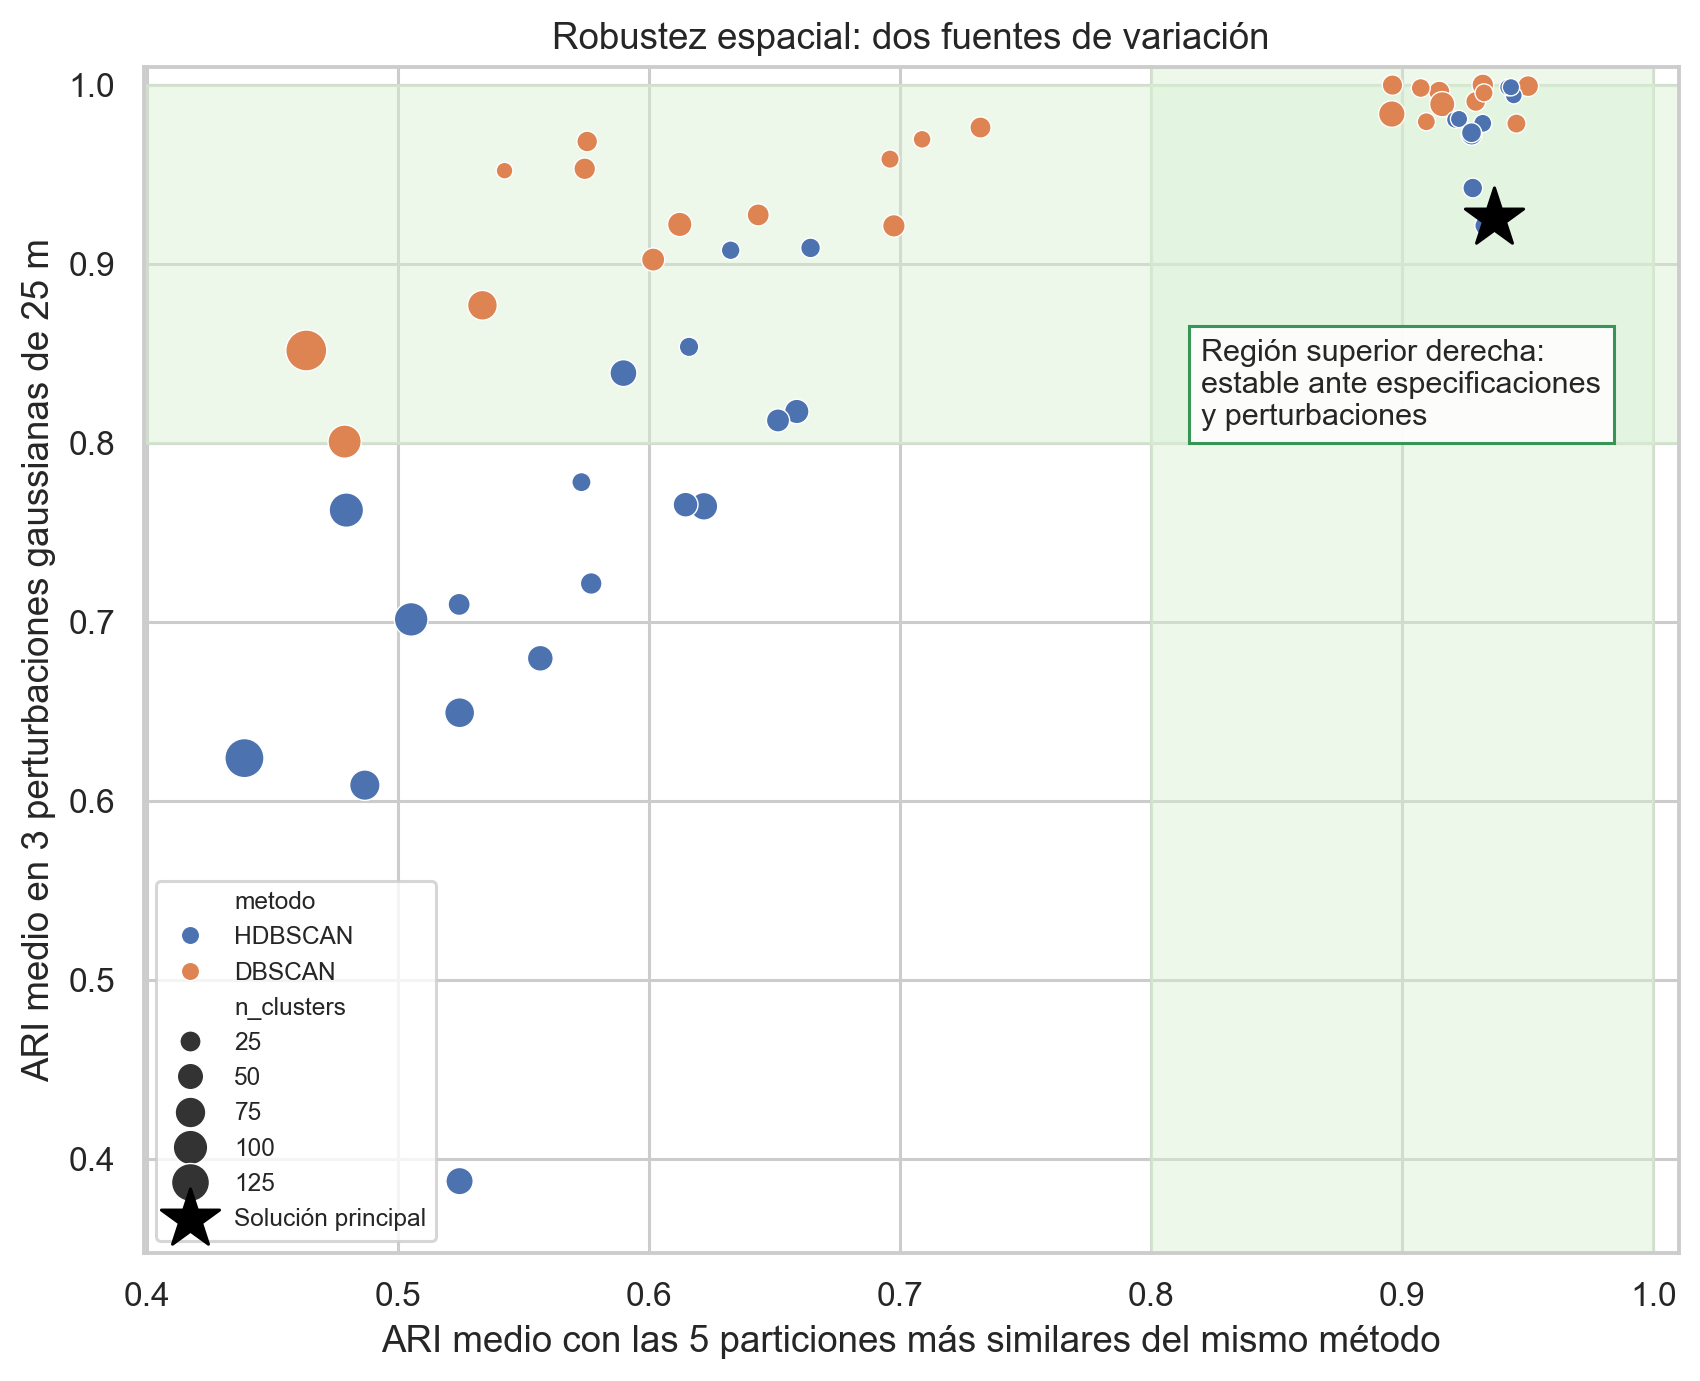
\includegraphics[width=.94\textwidth]{01_robustez_ari_documentada.png}\end{figure}
\section{ARI: definición, comparaciones y sensibilidad a grupos grandes}ARI compara particiones completas mediante pares de observaciones y corrige acuerdo por azar. ARI=1 indica identidad; cerca de 0, acuerdo equivalente al azar; valores bajos o negativos, desacuerdo. La comparación histórica es la media de las cinco particiones HDBSCAN con mayor ARI frente a la principal. La perturbación suma ruido gaussiano independiente de desviación 25 m a cada eje, reajusta HDBSCAN completo tres veces y promedia; semilla maestra 20260921. Para ``sin ruido'' se restringe a observaciones no ruido en ambas particiones. Para ``sin mega'' se excluyen las observaciones cuyo cluster principal es 20. {\scriptsize\setlength{\tabcolsep}{2pt}\begin{longtable}{>{\raggedright\arraybackslash}p{3.04cm}>{\raggedright\arraybackslash}p{3.04cm}>{\raggedright\arraybackslash}p{3.04cm}>{\raggedright\arraybackslash}p{3.04cm}>{\raggedright\arraybackslash}p{3.04cm}}\toprule Comparación & n & ARI global & ARI sin ruido & ARI sin mega\\\midrule\endhead cinco\_\allowbreak{}particiones\_\allowbreak{}mas\_\allowbreak{}similares\_\allowbreak{}mismo\_\allowbreak{}metodo & 5 & 0.937 & 0.992 & 0.819 \\
perturbacion\_\allowbreak{}gaussiana\_\allowbreak{}25m & 3 & 0.926 & 0.986 & 0.896 \\\bottomrule\end{longtable}} El descenso sin el mega-cluster confirma contribución de las categorías grandes, pero la estabilidad residual continúa alta en promedio; los mínimos completos están en \texttt{resumen\_ari\_variantes.csv}.
\section{Estabilidad de membresía entre especificaciones}Para cada cluster principal y cada una de cinco alternativas (DBSCAN de referencia y cuatro HDBSCAN de sensibilidad), se elige el cluster alternativo de Jaccard máximo. Para cada punto, $s_i$ es la fracción de alternativas donde permanece en ese emparejamiento; cada escenario pesa 0.2. Ruido se compara con ruido. Clases: sensible 0--.49; estable .50--.79; núcleo robusto .80--1. No es cohesión interna, densidad, probabilidad HDBSCAN ni persistencia nativa. \begin{figure}[H]\centering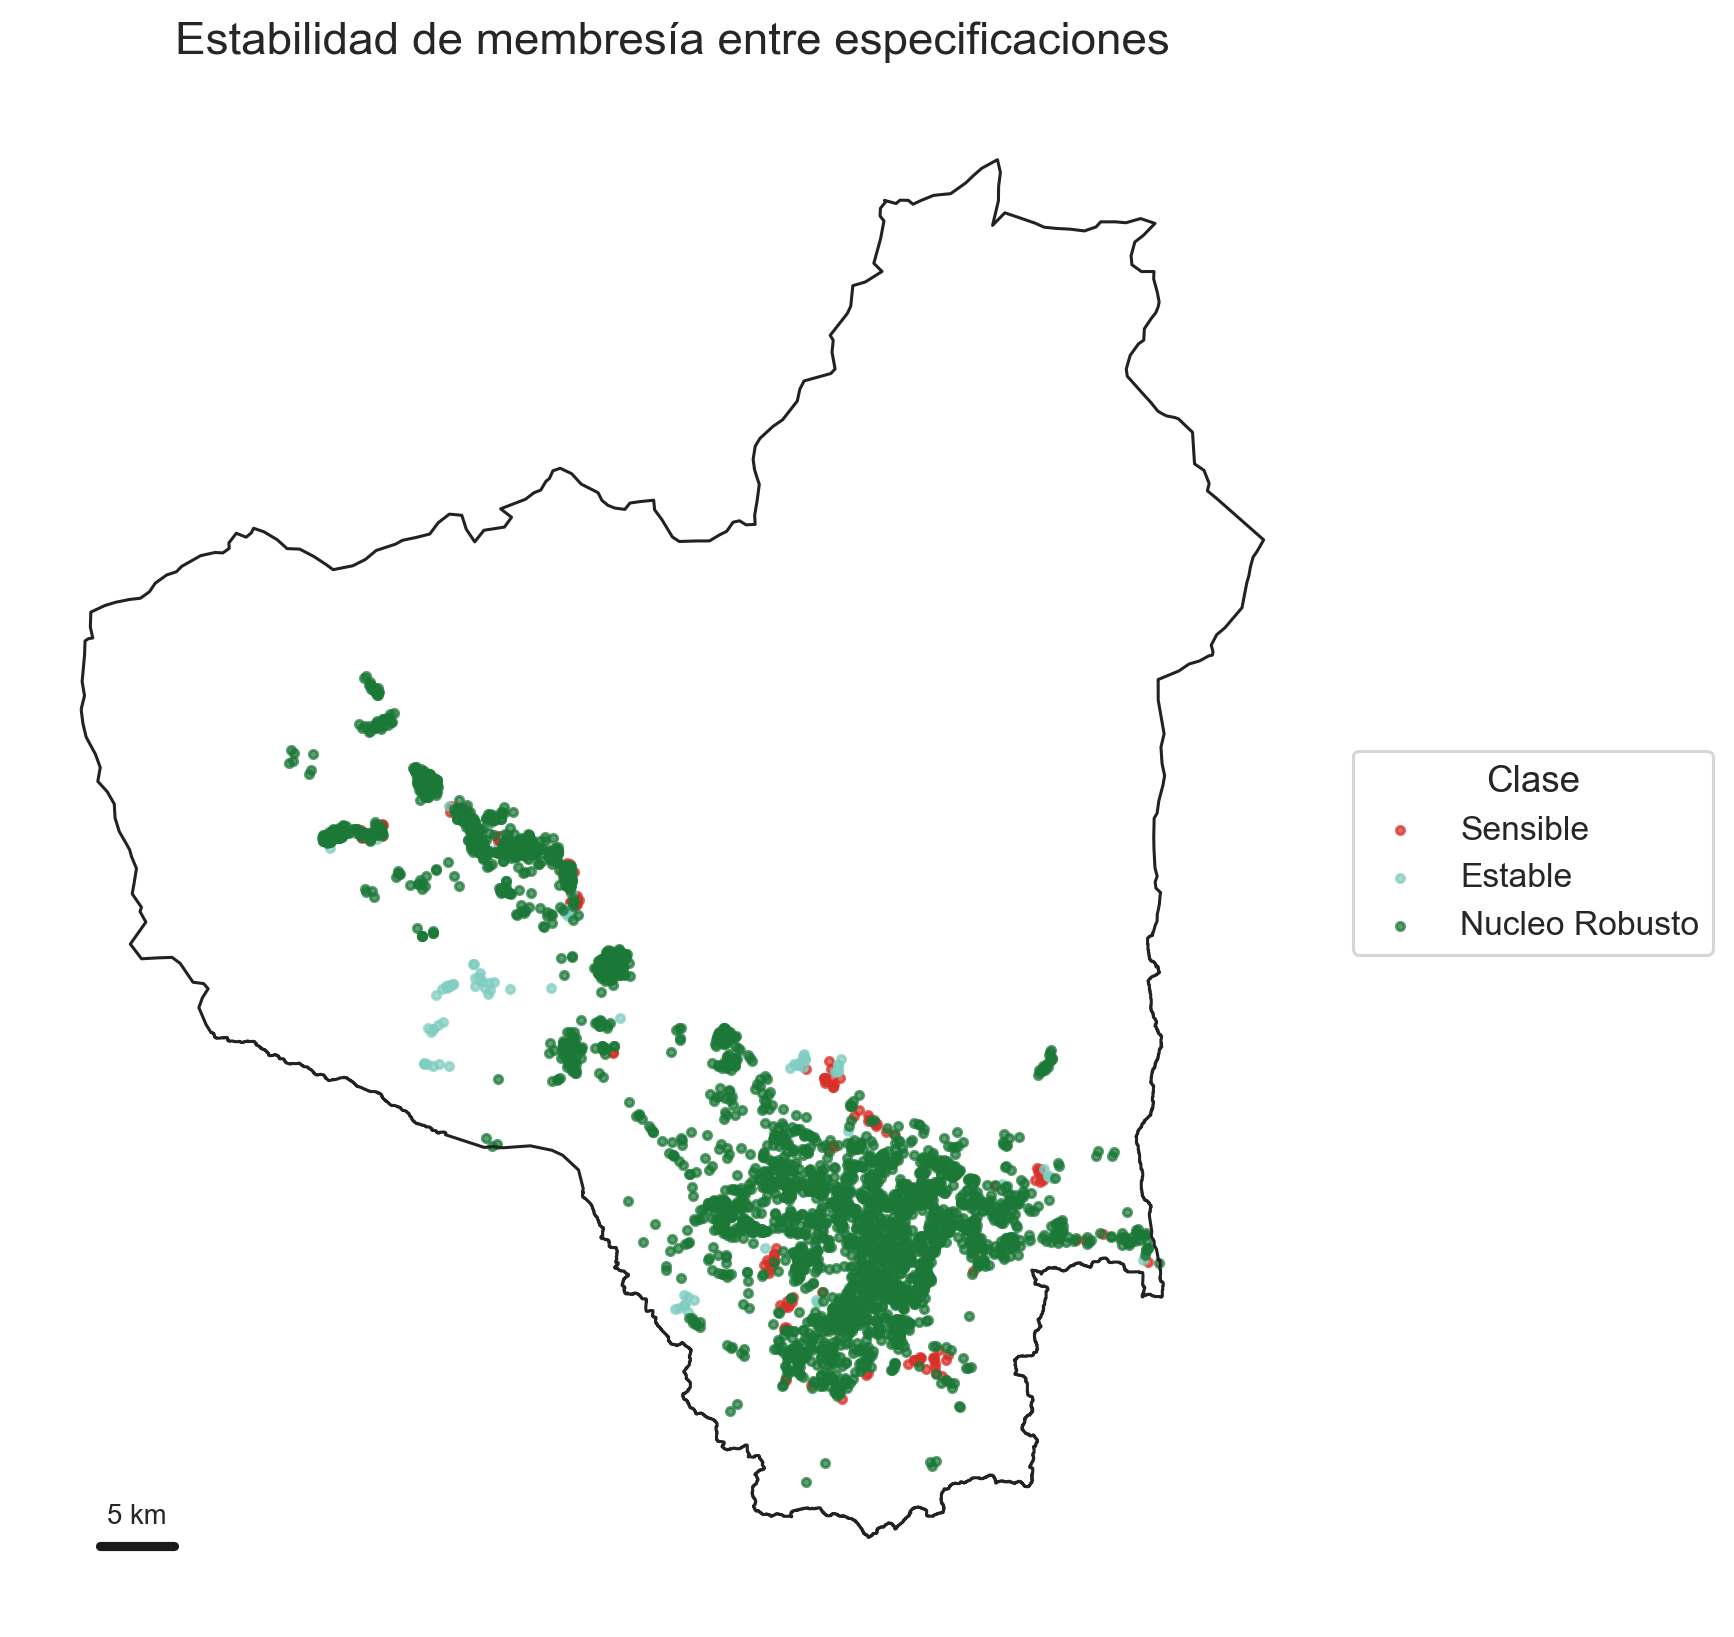
\includegraphics[width=.94\textwidth]{02_estabilidad_membresia.png}\end{figure} {\scriptsize\setlength{\tabcolsep}{2pt}\begin{longtable}{>{\raggedright\arraybackslash}p{1.90cm}>{\raggedright\arraybackslash}p{1.90cm}>{\raggedright\arraybackslash}p{1.90cm}>{\raggedright\arraybackslash}p{1.90cm}>{\raggedright\arraybackslash}p{1.90cm}>{\raggedright\arraybackslash}p{1.90cm}>{\raggedright\arraybackslash}p{1.90cm}>{\raggedright\arraybackslash}p{1.90cm}}\toprule Cl. & n & Estab. & Jacc. med. & Jacc. mín. & Robusto \% & Estable \% & Sensible \%\\\midrule\endhead 0.0 & 211.0 & 1.00 & 1.00 & 1.00 & 100.00 & 0.00 & 0.00 \\
1.0 & 41.0 & 0.98 & 0.98 & 0.90 & 100.00 & 0.00 & 0.00 \\
2.0 & 37.0 & 1.00 & 1.00 & 1.00 & 100.00 & 0.00 & 0.00 \\
3.0 & 20.0 & 0.40 & 0.40 & 0.00 & 0.00 & 0.00 & 100.00 \\
4.0 & 28.0 & 0.60 & 0.51 & 0.00 & 0.00 & 100.00 & 0.00 \\
5.0 & 33.0 & 1.00 & 0.84 & 0.62 & 100.00 & 0.00 & 0.00 \\
6.0 & 20.0 & 0.82 & 0.56 & 0.04 & 100.00 & 0.00 & 0.00 \\
7.0 & 99.0 & 0.99 & 0.97 & 0.92 & 100.00 & 0.00 & 0.00 \\
8.0 & 337.0 & 1.00 & 1.00 & 1.00 & 100.00 & 0.00 & 0.00 \\
9.0 & 30.0 & 0.97 & 0.70 & 0.16 & 93.33 & 6.67 & 0.00 \\
10.0 & 142.0 & 0.99 & 0.94 & 0.74 & 98.59 & 1.41 & 0.00 \\
11.0 & 48.0 & 0.97 & 0.91 & 0.83 & 100.00 & 0.00 & 0.00 \\
12.0 & 224.0 & 1.00 & 0.86 & 0.31 & 99.55 & 0.45 & 0.00 \\
13.0 & 149.0 & 1.00 & 0.82 & 0.21 & 99.33 & 0.67 & 0.00 \\
14.0 & 14.0 & 0.40 & 0.19 & 0.00 & 0.00 & 0.00 & 100.00 \\
15.0 & 92.0 & 0.98 & 0.76 & 0.13 & 94.57 & 5.43 & 0.00 \\
16.0 & 51.0 & 0.98 & 0.71 & 0.07 & 100.00 & 0.00 & 0.00 \\
17.0 & 45.0 & 1.00 & 0.80 & 0.06 & 100.00 & 0.00 & 0.00 \\
18.0 & 32.0 & 0.97 & 0.89 & 0.76 & 93.75 & 3.12 & 3.12 \\
19.0 & 100.0 & 0.93 & 0.91 & 0.67 & 100.00 & 0.00 & 0.00 \\
20.0 & 1997.0 & 1.00 & 0.97 & 0.92 & 99.65 & 0.35 & 0.00 \\
21.0 & 31.0 & 0.99 & 0.78 & 0.01 & 96.77 & 3.23 & 0.00 \\\bottomrule\end{longtable}}
\section{Mega-cluster 20 y 18 subnúcleos exploratorios}El diagnóstico interno usa sólo coordenadas con HDBSCAN \texttt{min\_cluster\_size=30}, \texttt{min\_samples=10}, método leaf. Leaf favorece ramas locales con tamaño suficiente y se usa para revelar heterogeneidad, no para reemplazar el cluster 20. El 44.5\% no asignado significa que esos puntos no pertenecen a una rama local suficientemente densa bajo esta especificación; siguen perteneciendo al cluster principal. \begin{figure}[H]\centering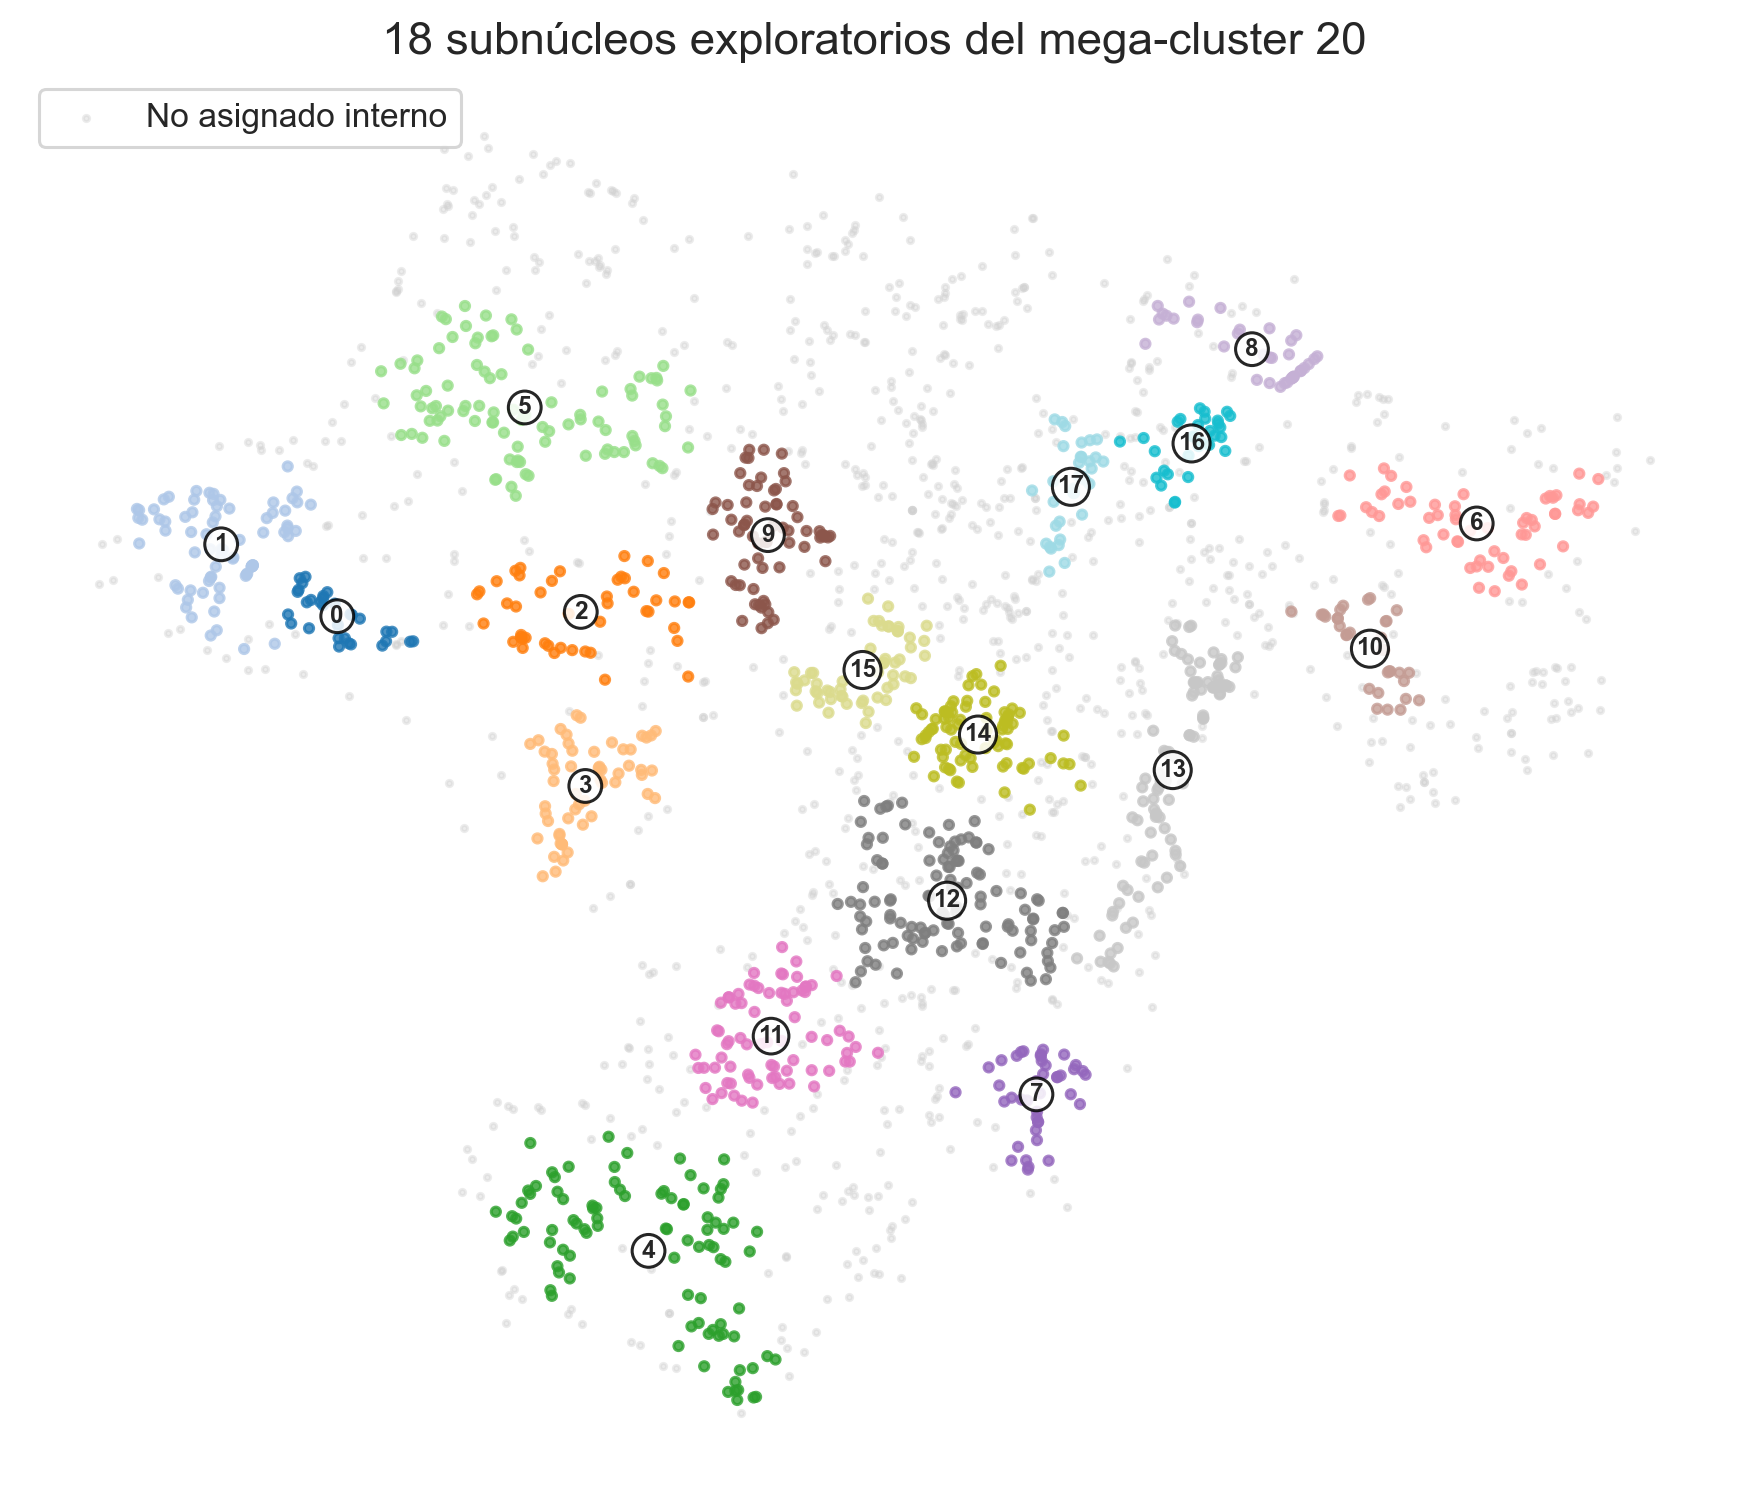
\includegraphics[width=.94\textwidth]{03_subnucleos_mega_etiquetados.png}\end{figure}\subsection{Geometría}Área convexa y densidad son descriptivas; el medoide es un establecimiento observado y la distancia vecina se mide entre centroides. {\scriptsize\setlength{\tabcolsep}{2pt}\begin{longtable}{>{\raggedright\arraybackslash}p{1.69cm}>{\raggedright\arraybackslash}p{1.69cm}>{\raggedright\arraybackslash}p{1.69cm}>{\raggedright\arraybackslash}p{1.69cm}>{\raggedright\arraybackslash}p{1.69cm}>{\raggedright\arraybackslash}p{1.69cm}>{\raggedright\arraybackslash}p{1.69cm}>{\raggedright\arraybackslash}p{1.69cm}>{\raggedright\arraybackslash}p{1.69cm}}\toprule ID & n & \% mega & Municipio & Localidad & Área km2 & Dens./km2 & Loc. & Vecino m\\\midrule\endhead 0 & 31 & 1.6 & San Andrés Cholula & San Andrés Cholula & 0.9 & 34.9 & 1 & 1949.8 \\
1 & 76 & 3.8 & San Pedro Cholula & Cholula de Rivadavia & 4.4 & 17.3 & 2 & 1949.8 \\
2 & 46 & 2.3 & Puebla & Heroica Puebla de Zaragoza & 4.1 & 11.1 & 3 & 2513.7 \\
3 & 57 & 2.9 & San Andrés Cholula & San Bernardino Tlaxcalancingo & 2.9 & 19.6 & 1 & 2513.7 \\
4 & 92 & 4.6 & Puebla & Heroica Puebla de Zaragoza & 9.9 & 9.3 & 1 & 3571.9 \\
5 & 93 & 4.7 & San Pedro Cholula & Santiago Momoxpan & 8.4 & 11.1 & 5 & 3060.4 \\
6 & 58 & 2.9 & Puebla & Heroica Puebla de Zaragoza & 4.5 & 12.8 & 1 & 2389.7 \\
7 & 41 & 2.1 & Puebla & Heroica Puebla de Zaragoza & 2.0 & 20.3 & 1 & 3086.9 \\
8 & 36 & 1.8 & Puebla & Heroica Puebla de Zaragoza & 1.7 & 20.7 & 1 & 1615.8 \\
9 & 65 & 3.3 & Puebla & Heroica Puebla de Zaragoza & 2.9 & 22.7 & 1 & 2378.4 \\
10 & 33 & 1.7 & Puebla & Heroica Puebla de Zaragoza & 1.7 & 19.9 & 1 & 2389.7 \\
11 & 74 & 3.7 & Puebla & Heroica Puebla de Zaragoza & 3.8 & 19.7 & 1 & 3204.8 \\
12 & 112 & 5.6 & Puebla & Heroica Puebla de Zaragoza & 6.6 & 17.1 & 1 & 2436.5 \\
13 & 97 & 4.9 & Puebla & Heroica Puebla de Zaragoza & 4.7 & 20.7 & 1 & 2858.1 \\
14 & 78 & 3.9 & Puebla & Heroica Puebla de Zaragoza & 3.2 & 24.4 & 1 & 1909.9 \\
15 & 54 & 2.7 & Puebla & Heroica Puebla de Zaragoza & 2.2 & 25.0 & 1 & 1909.9 \\
16 & 30 & 1.5 & Puebla & Heroica Puebla de Zaragoza & 1.2 & 25.3 & 1 & 1615.8 \\
17 & 35 & 1.8 & Puebla & Heroica Puebla de Zaragoza & 1.3 & 26.3 & 1 & 1850.7 \\\bottomrule\end{longtable}}\subsection{Perfilado económico posterior}Las siguientes variables se agregan después del diagnóstico espacial y no generaron los subnúcleos. {\scriptsize\setlength{\tabcolsep}{2pt}\begin{longtable}{>{\raggedright\arraybackslash}p{1.38cm}>{\raggedright\arraybackslash}p{1.38cm}>{\raggedright\arraybackslash}p{1.38cm}>{\raggedright\arraybackslash}p{1.38cm}>{\raggedright\arraybackslash}p{1.38cm}>{\raggedright\arraybackslash}p{1.38cm}>{\raggedright\arraybackslash}p{1.38cm}>{\raggedright\arraybackslash}p{1.38cm}>{\raggedright\arraybackslash}p{1.38cm}>{\raggedright\arraybackslash}p{1.38cm}>{\raggedright\arraybackslash}p{1.38cm}}\toprule ID & Man. & Lav. & Conf. & Acab. & Telas & Maq. & Mez./pant. & Húm. & Seco & SCIAN-3\\\midrule\endhead 0 & 16.1 & 83.9 & 9.7 & 0.0 & 0.0 & 3.2 & 0.0 & 16.1 & 0.0 & 812 | 315 \\
1 & 40.8 & 59.2 & 15.8 & 1.3 & 3.9 & 1.3 & 0.0 & 19.7 & 6.6 & 812 | 315 | 313 \\
2 & 19.6 & 80.4 & 6.5 & 0.0 & 0.0 & 0.0 & 0.0 & 23.9 & 6.5 & 812 | 315 | 314 \\
3 & 24.6 & 75.4 & 14.0 & 0.0 & 3.5 & 1.8 & 0.0 & 19.3 & 3.5 & 812 | 315 | 313 \\
4 & 41.3 & 58.7 & 30.4 & 0.0 & 1.1 & 4.3 & 0.0 & 6.5 & 12.0 & 812 | 315 | 314 \\
5 & 43.0 & 57.0 & 17.2 & 3.2 & 7.5 & 4.3 & 0.0 & 12.9 & 7.5 & 812 | 315 | 314 \\
6 & 39.7 & 60.3 & 25.9 & 0.0 & 0.0 & 3.4 & 0.0 & 15.5 & 10.3 & 812 | 315 | 314 \\
7 & 41.5 & 58.5 & 24.4 & 0.0 & 0.0 & 2.4 & 0.0 & 14.6 & 7.3 & 812 | 315 | 313 \\
8 & 50.0 & 50.0 & 8.3 & 5.6 & 19.4 & 5.6 & 0.0 & 5.6 & 0.0 & 812 | 313 | 315 \\
9 & 46.2 & 53.8 & 18.5 & 0.0 & 7.7 & 4.6 & 0.0 & 10.8 & 10.8 & 812 | 315 | 313 \\
10 & 42.4 & 57.6 & 30.3 & 0.0 & 3.0 & 0.0 & 3.0 & 24.2 & 12.1 & 812 | 315 | 314 \\
11 & 40.5 & 59.5 & 33.8 & 0.0 & 1.4 & 0.0 & 0.0 & 16.2 & 13.5 & 812 | 315 | 314 \\
12 & 39.3 & 60.7 & 14.3 & 0.9 & 5.4 & 2.7 & 0.0 & 16.1 & 4.5 & 812 | 315 | 314 \\
13 & 55.7 & 44.3 & 19.6 & 2.1 & 10.3 & 2.1 & 0.0 & 14.4 & 12.4 & 812 | 315 | 313 \\
14 & 60.3 & 39.7 & 37.2 & 0.0 & 1.3 & 0.0 & 0.0 & 19.2 & 11.5 & 812 | 315 | 314 \\
15 & 29.6 & 70.4 & 25.9 & 1.9 & 1.9 & 1.9 & 0.0 & 13.0 & 1.9 & 812 | 315 | 313 \\
16 & 70.0 & 30.0 & 36.7 & 3.3 & 10.0 & 0.0 & 0.0 & 10.0 & 16.7 & 315 | 812 | 313 \\
17 & 37.1 & 62.9 & 17.1 & 0.0 & 11.4 & 0.0 & 0.0 & 14.3 & 17.1 & 812 | 315 | 313 \\\bottomrule\end{longtable}}
\section{Composición multilabel y diccionario analítico}Los términos son cadenas disparadoras; las etiquetas canónicas son indicadores reproducibles derivados; las categorías agregadas reúnen reglas como SCIAN o señales temáticas. El heatmap principal conserva ocho variables centrales, interpretables y poco redundantes; el ampliado muestra las 18 variables útiles. Ninguno incluye miles de términos crudos. La trazabilidad completa está en \texttt{diccionario\_variables\_analiticas.csv}. \begin{figure}[H]\centering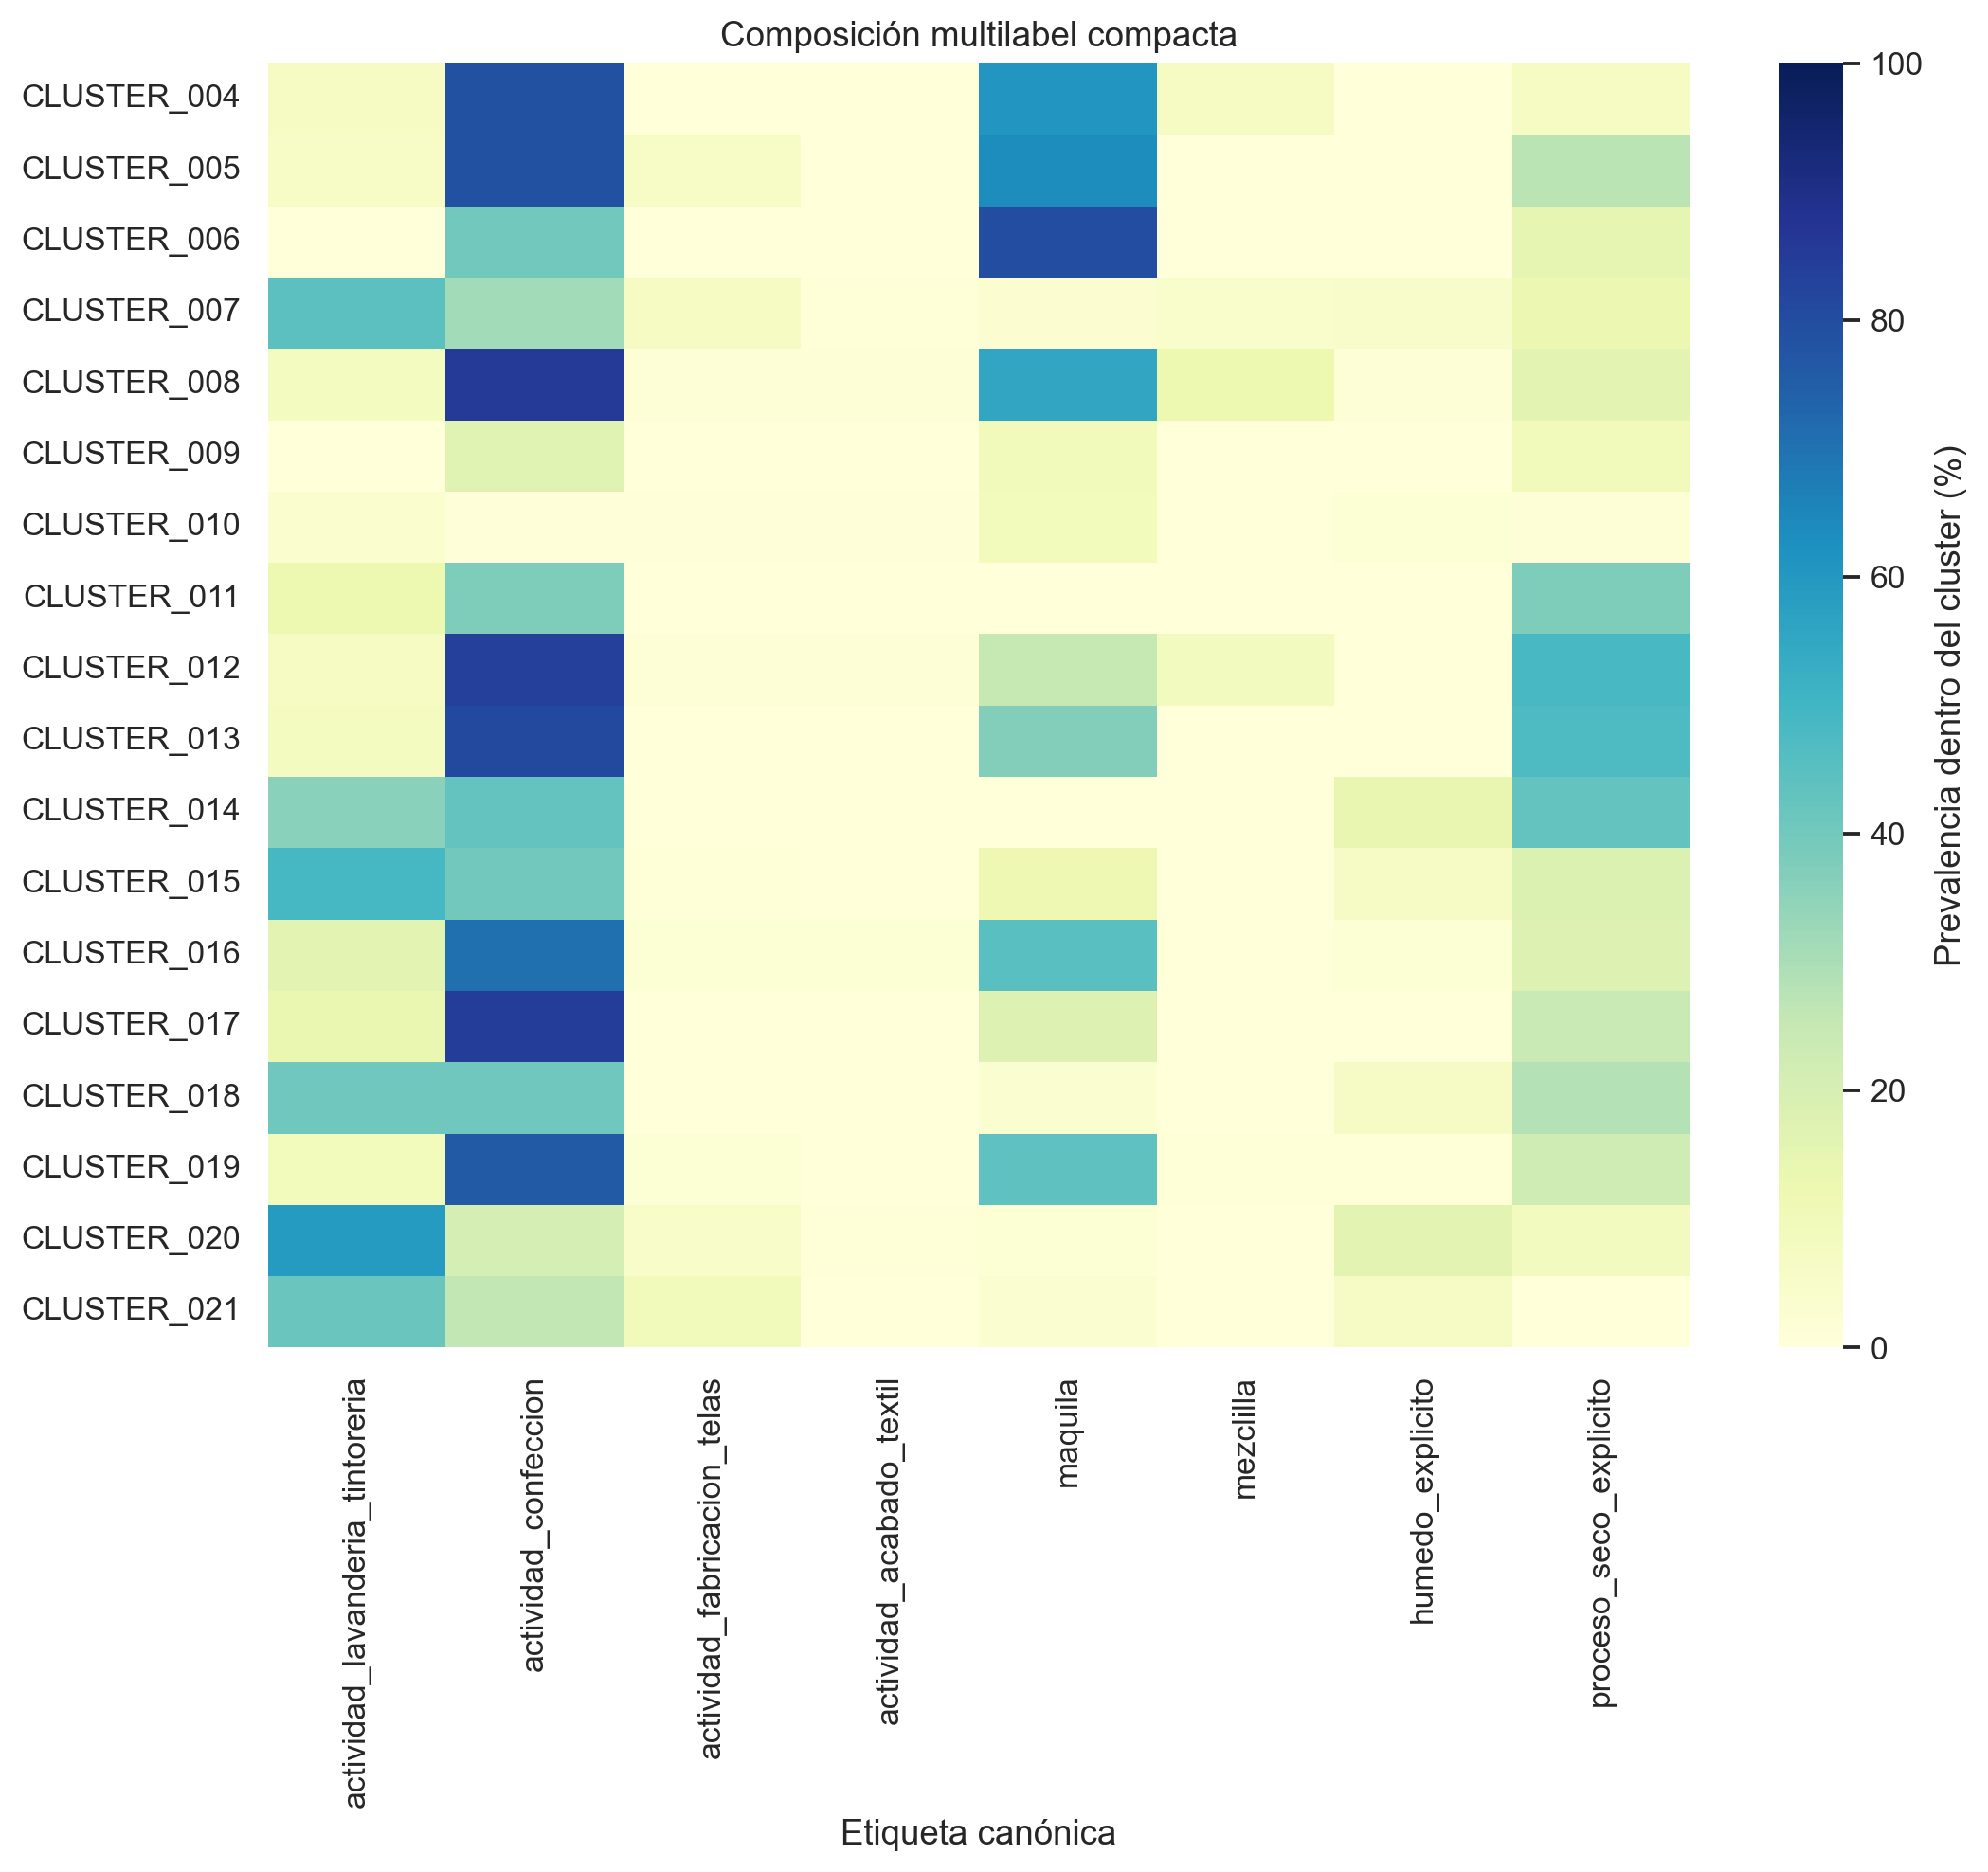
\includegraphics[width=.94\textwidth]{04_heatmap_compacto.png}\end{figure} \begin{figure}[H]\centering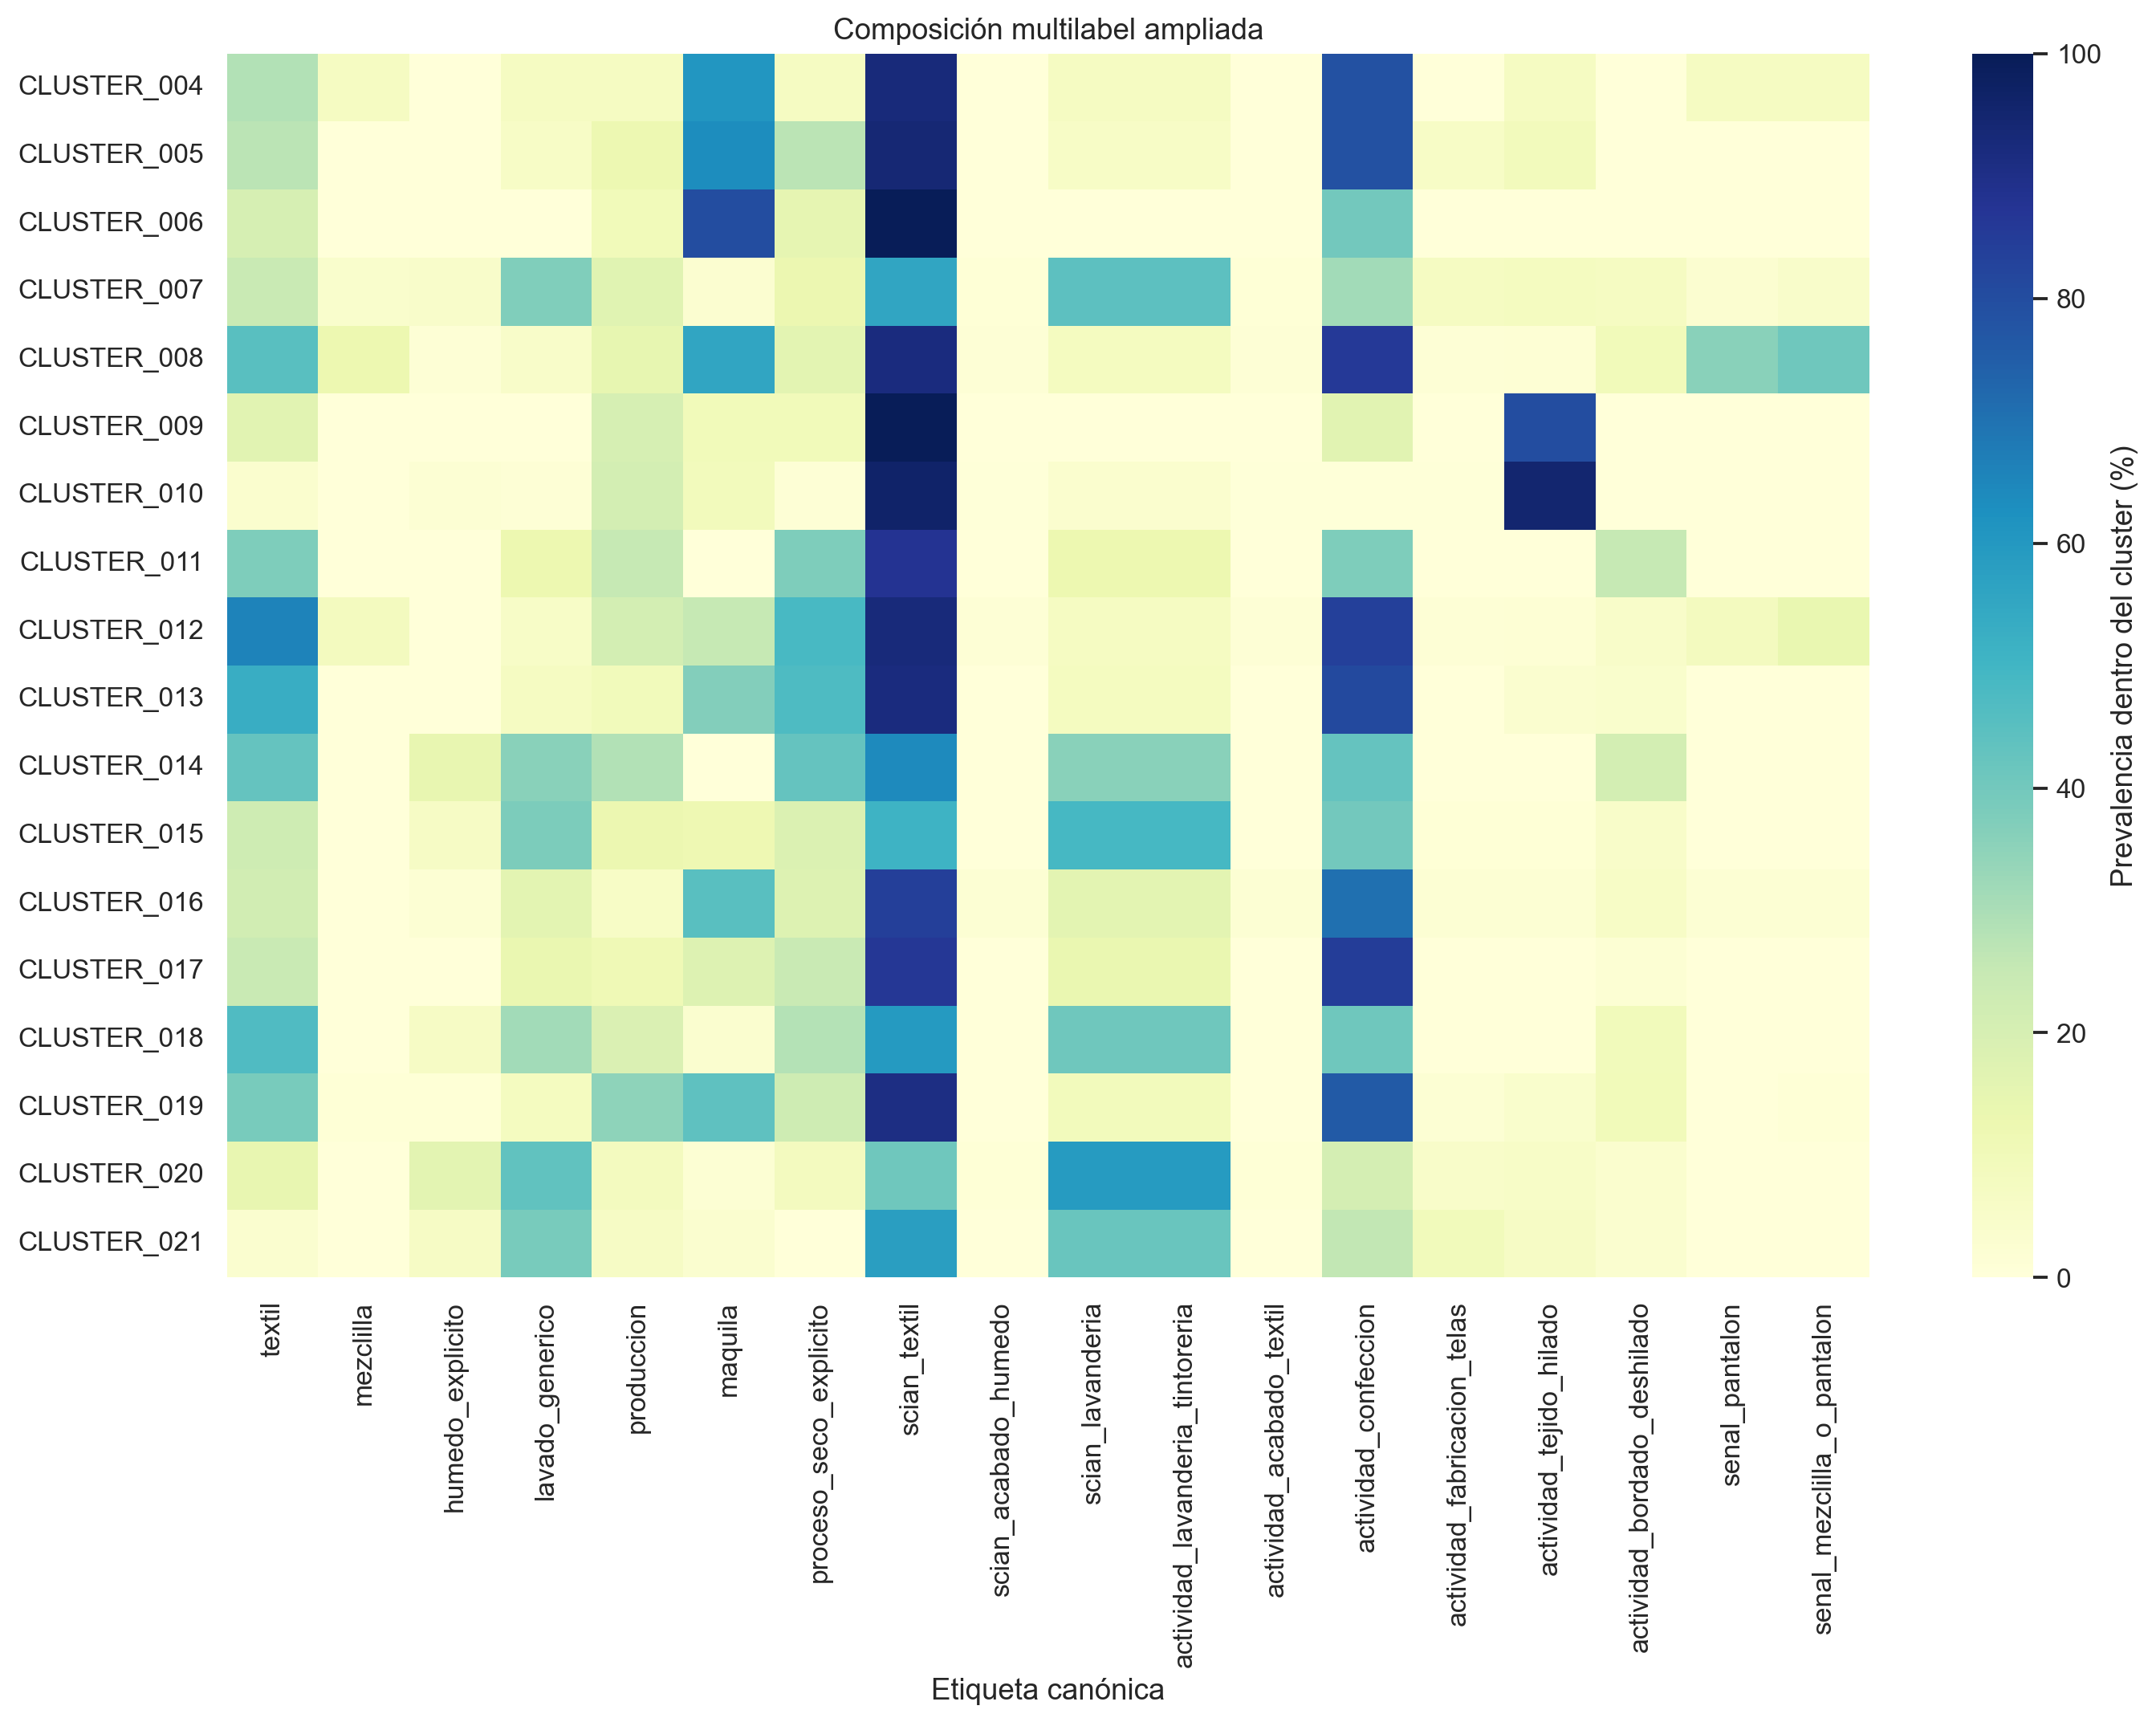
\includegraphics[width=.94\textwidth]{05_heatmap_ampliado.png}\end{figure}
\section{Sobrerrepresentación}Una señal está sobrerrepresentada cuando $p_c>p_U$. $lift=p_c/p_U$ y $\log_2(lift)=\log_2(p_c/p_U)$: cero significa igualdad; positivo, sobre-representación; negativo, subrepresentación. Se distingue \texttt{NO\_EVALUABLE} (base global cero), \texttt{NO\_SOBRERREPRESENTADO} (lift $\le1$), \texttt{FILTRADO\_POR\_CRITERIO} y \texttt{SOBRERREPRESENTADO}. El filtro exige conteo $\ge5$, prevalencia $\ge5\%$, lift $\ge1.25$ y $p_{BH}\le.05$. La tabla completa contiene conteo, prevalencias, diferencia en puntos porcentuales, lift, log2 lift, OR, IC95, Fisher y BH; \texttt{top\_rasgos\_por\_cluster.csv} aporta 3--5 rasgos por cluster cuando existen.
\section{Lavanderías frente a manufactura}El 80\% es un umbral descriptivo, no una frontera natural. En la referencia fija hay 12 concentraciones manufactureras y seis mixtas; ninguna predominantemente lavandería. \begin{figure}[H]\centering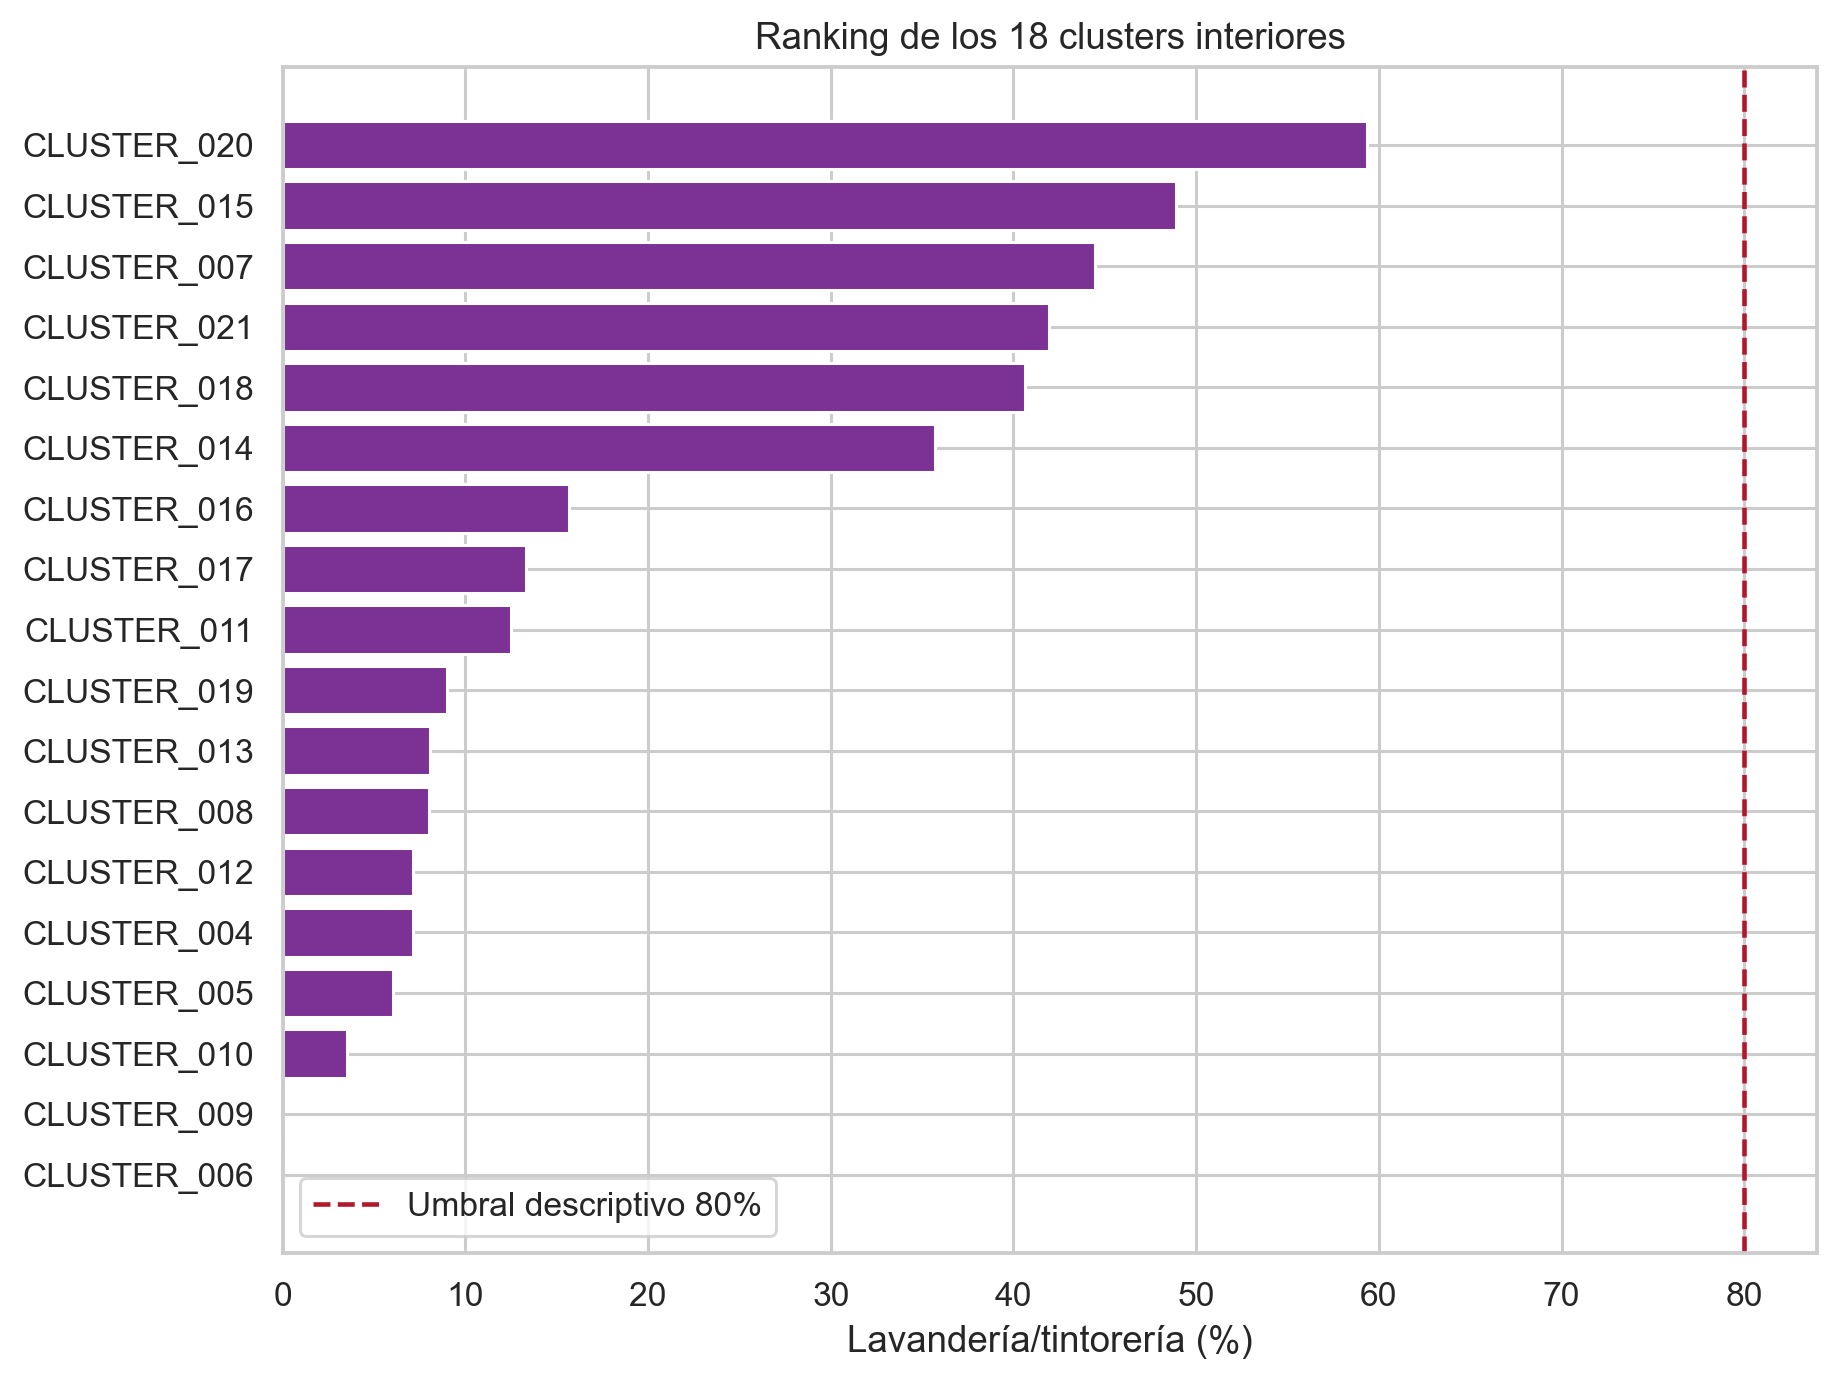
\includegraphics[width=.94\textwidth]{08_ranking_lavanderia.png}\end{figure} {\scriptsize\setlength{\tabcolsep}{2pt}\begin{longtable}{>{\raggedright\arraybackslash}p{1.27cm}>{\raggedright\arraybackslash}p{1.27cm}>{\raggedright\arraybackslash}p{1.27cm}>{\raggedright\arraybackslash}p{1.27cm}>{\raggedright\arraybackslash}p{1.27cm}>{\raggedright\arraybackslash}p{1.27cm}>{\raggedright\arraybackslash}p{1.27cm}>{\raggedright\arraybackslash}p{1.27cm}>{\raggedright\arraybackslash}p{1.27cm}>{\raggedright\arraybackslash}p{1.27cm}>{\raggedright\arraybackslash}p{1.27cm}>{\raggedright\arraybackslash}p{1.27cm}}\toprule Cl. & n & Municipio & Localidad & Lav. & Man. & Conf. & Acab. & Maq. & Húm. & Seco & Mez./pant.\\\midrule\endhead 20 & 1997 & Puebla & Heroica Puebla de Zaragoza & 59.3 & 40.7 & 20.9 & 1.0 & 2.2 & 15.7 & 8.5 & 0.2 \\
15 & 92 & San Martín Texmelucan & San Martín Texmelucan de Labastida & 48.9 & 51.1 & 40.2 & 0.0 & 12.0 & 6.5 & 18.5 & 0.0 \\
7 & 99 & Huejotzingo & Huejotzingo & 44.4 & 55.6 & 31.3 & 1.0 & 3.0 & 5.1 & 13.1 & 5.1 \\
21 & 31 & Amozoc & Amozoc de Mota & 41.9 & 58.1 & 25.8 & 0.0 & 3.2 & 6.5 & 0.0 & 0.0 \\
18 & 32 & Amozoc & Amozoc de Mota & 40.6 & 59.4 & 40.6 & 0.0 & 3.1 & 6.2 & 28.1 & 0.0 \\
14 & 14 & Cuautlancingo & San Lorenzo Almecatla & 35.7 & 64.3 & 42.9 & 0.0 & 0.0 & 14.3 & 42.9 & 0.0 \\
16 & 51 & San Martín Texmelucan & Santa María Moyotzingo & 15.7 & 84.3 & 70.6 & 2.0 & 45.1 & 2.0 & 17.6 & 2.0 \\
17 & 45 & San Martín Texmelucan & San Martín Texmelucan de Labastida & 13.3 & 86.7 & 84.4 & 0.0 & 17.8 & 0.0 & 24.4 & 0.0 \\
11 & 8 & Ocoyucan & San Bernabé Temoxtitla & 12.5 & 87.5 & 37.5 & 0.0 & 0.0 & 0.0 & 37.5 & 0.0 \\
19 & 100 & San Miguel Xoxtla & San Miguel Xoxtla & 9.0 & 91.0 & 76.0 & 0.0 & 44.0 & 1.0 & 23.0 & 1.0 \\
13 & 149 & San Martín Texmelucan & San Rafael Tlanalapan & 8.1 & 91.9 & 81.2 & 0.0 & 36.9 & 0.0 & 47.7 & 0.0 \\
8 & 337 & Huejotzingo & Santa Ana Xalmimilulco & 8.0 & 92.0 & 85.8 & 1.2 & 55.8 & 1.5 & 15.7 & 40.7 \\
12 & 224 & San Matías Tlalancaleca & San Matías Tlalancaleca & 7.1 & 92.9 & 83.9 & 1.3 & 25.0 & 0.0 & 48.7 & 13.8 \\
4 & 28 & Chiautzingo & San Lorenzo Chiautzingo & 7.1 & 92.9 & 78.6 & 0.0 & 60.7 & 0.0 & 7.1 & 7.1 \\
5 & 33 & San Matías Tlalancaleca & Juárez Coronaco & 6.1 & 93.9 & 78.8 & 0.0 & 63.6 & 0.0 & 27.3 & 0.0 \\
10 & 142 & Tlahuapan & San Rafael Ixtapalucan & 3.5 & 96.5 & 0.7 & 0.7 & 9.2 & 2.1 & 1.4 & 0.0 \\
6 & 20 & Tlahuapan & Santiago Coltzingo & 0.0 & 100.0 & 40.0 & 0.0 & 80.0 & 0.0 & 15.0 & 0.0 \\
9 & 30 & Tlahuapan & San Miguel Tianguistenco & 0.0 & 100.0 & 16.7 & 0.0 & 10.0 & 0.0 & 10.0 & 0.0 \\\bottomrule\end{longtable}} \subsection{Sensibilidad en seis escenarios}{\scriptsize\setlength{\tabcolsep}{2pt}\begin{longtable}{>{\raggedright\arraybackslash}p{2.17cm}>{\raggedright\arraybackslash}p{2.17cm}>{\raggedright\arraybackslash}p{2.17cm}>{\raggedright\arraybackslash}p{2.17cm}>{\raggedright\arraybackslash}p{2.17cm}>{\raggedright\arraybackslash}p{2.17cm}>{\raggedright\arraybackslash}p{2.17cm}}\toprule escenario\_\allowbreak{}id & rol & n\_\allowbreak{}clusters\_\allowbreak{}interiores & max\_\allowbreak{}pct\_\allowbreak{}lavanderias & clusters\_\allowbreak{}lavanderias\_\allowbreak{}80pct & clusters\_\allowbreak{}manufactura\_\allowbreak{}80pct & clusters\_\allowbreak{}coexistencia\_\allowbreak{}mixta\\\midrule\endhead hdbscan\_\allowbreak{}\_\allowbreak{}min\_\allowbreak{}cluster\_\allowbreak{}size-10\_\allowbreak{}\_\allowbreak{}min\_\allowbreak{}samples-20\_\allowbreak{}\_\allowbreak{}cluster\_\allowbreak{}selection\_\allowbreak{}method-eom & PRINCIPAL & 18 & 59.33900851276916 & 0 & 12 & 6 \\
dbscan\_\allowbreak{}\_\allowbreak{}eps\_\allowbreak{}m-1600\_\allowbreak{}\_\allowbreak{}min\_\allowbreak{}samples-25 & REFERENCIA\_\allowbreak{}DBSCAN & 9 & 58.21854912764004 & 0 & 5 & 4 \\
hdbscan\_\allowbreak{}\_\allowbreak{}min\_\allowbreak{}cluster\_\allowbreak{}size-20\_\allowbreak{}\_\allowbreak{}min\_\allowbreak{}samples-20\_\allowbreak{}\_\allowbreak{}cluster\_\allowbreak{}selection\_\allowbreak{}method-eom & SENSIBILIDAD & 17 & 59.33900851276916 & 0 & 12 & 5 \\
hdbscan\_\allowbreak{}\_\allowbreak{}min\_\allowbreak{}cluster\_\allowbreak{}size-30\_\allowbreak{}\_\allowbreak{}min\_\allowbreak{}samples-20\_\allowbreak{}\_\allowbreak{}cluster\_\allowbreak{}selection\_\allowbreak{}method-eom & SENSIBILIDAD & 15 & 59.33900851276916 & 0 & 10 & 5 \\
hdbscan\_\allowbreak{}\_\allowbreak{}min\_\allowbreak{}cluster\_\allowbreak{}size-20\_\allowbreak{}\_\allowbreak{}min\_\allowbreak{}samples-10\_\allowbreak{}\_\allowbreak{}cluster\_\allowbreak{}selection\_\allowbreak{}method-eom & SENSIBILIDAD & 20 & 58.93462469733656 & 0 & 13 & 7 \\
hdbscan\_\allowbreak{}\_\allowbreak{}min\_\allowbreak{}cluster\_\allowbreak{}size-30\_\allowbreak{}\_\allowbreak{}min\_\allowbreak{}samples-10\_\allowbreak{}\_\allowbreak{}cluster\_\allowbreak{}selection\_\allowbreak{}method-eom & SENSIBILIDAD & 17 & 58.93462469733656 & 0 & 10 & 7 \\\bottomrule\end{longtable}} La evidencia responde: las lavanderías no forman clusters interiores casi exclusivos; aparecen sobre todo en estructuras mixtas y coexisten con confección, acabado, maquila y señales textiles en proporciones variables. La conclusión permanece en los seis escenarios seleccionados. Esto no demuestra relación empresarial, productiva o hidráulica.
\section{Tipología y espacio métrico}El vector coseno contiene prevalencias (0--1) de las 18 etiquetas canónicas. Se usa distancia, $1-(x\cdot y)/(\|x\|\|y\|)$. Jensen--Shannon usa distribuciones SCIAN de 3 dígitos normalizadas por cluster y la distancia (raíz de la divergencia, base 2) implementada por SciPy. Personal ocupado aparece en el archivo de vectores histórico, pero no interviene en la distancia. La distancia final es $.5d_{cos}+.5d_{JS}$, sin normalización adicional porque ambas están en 0--1. \begin{figure}[H]\centering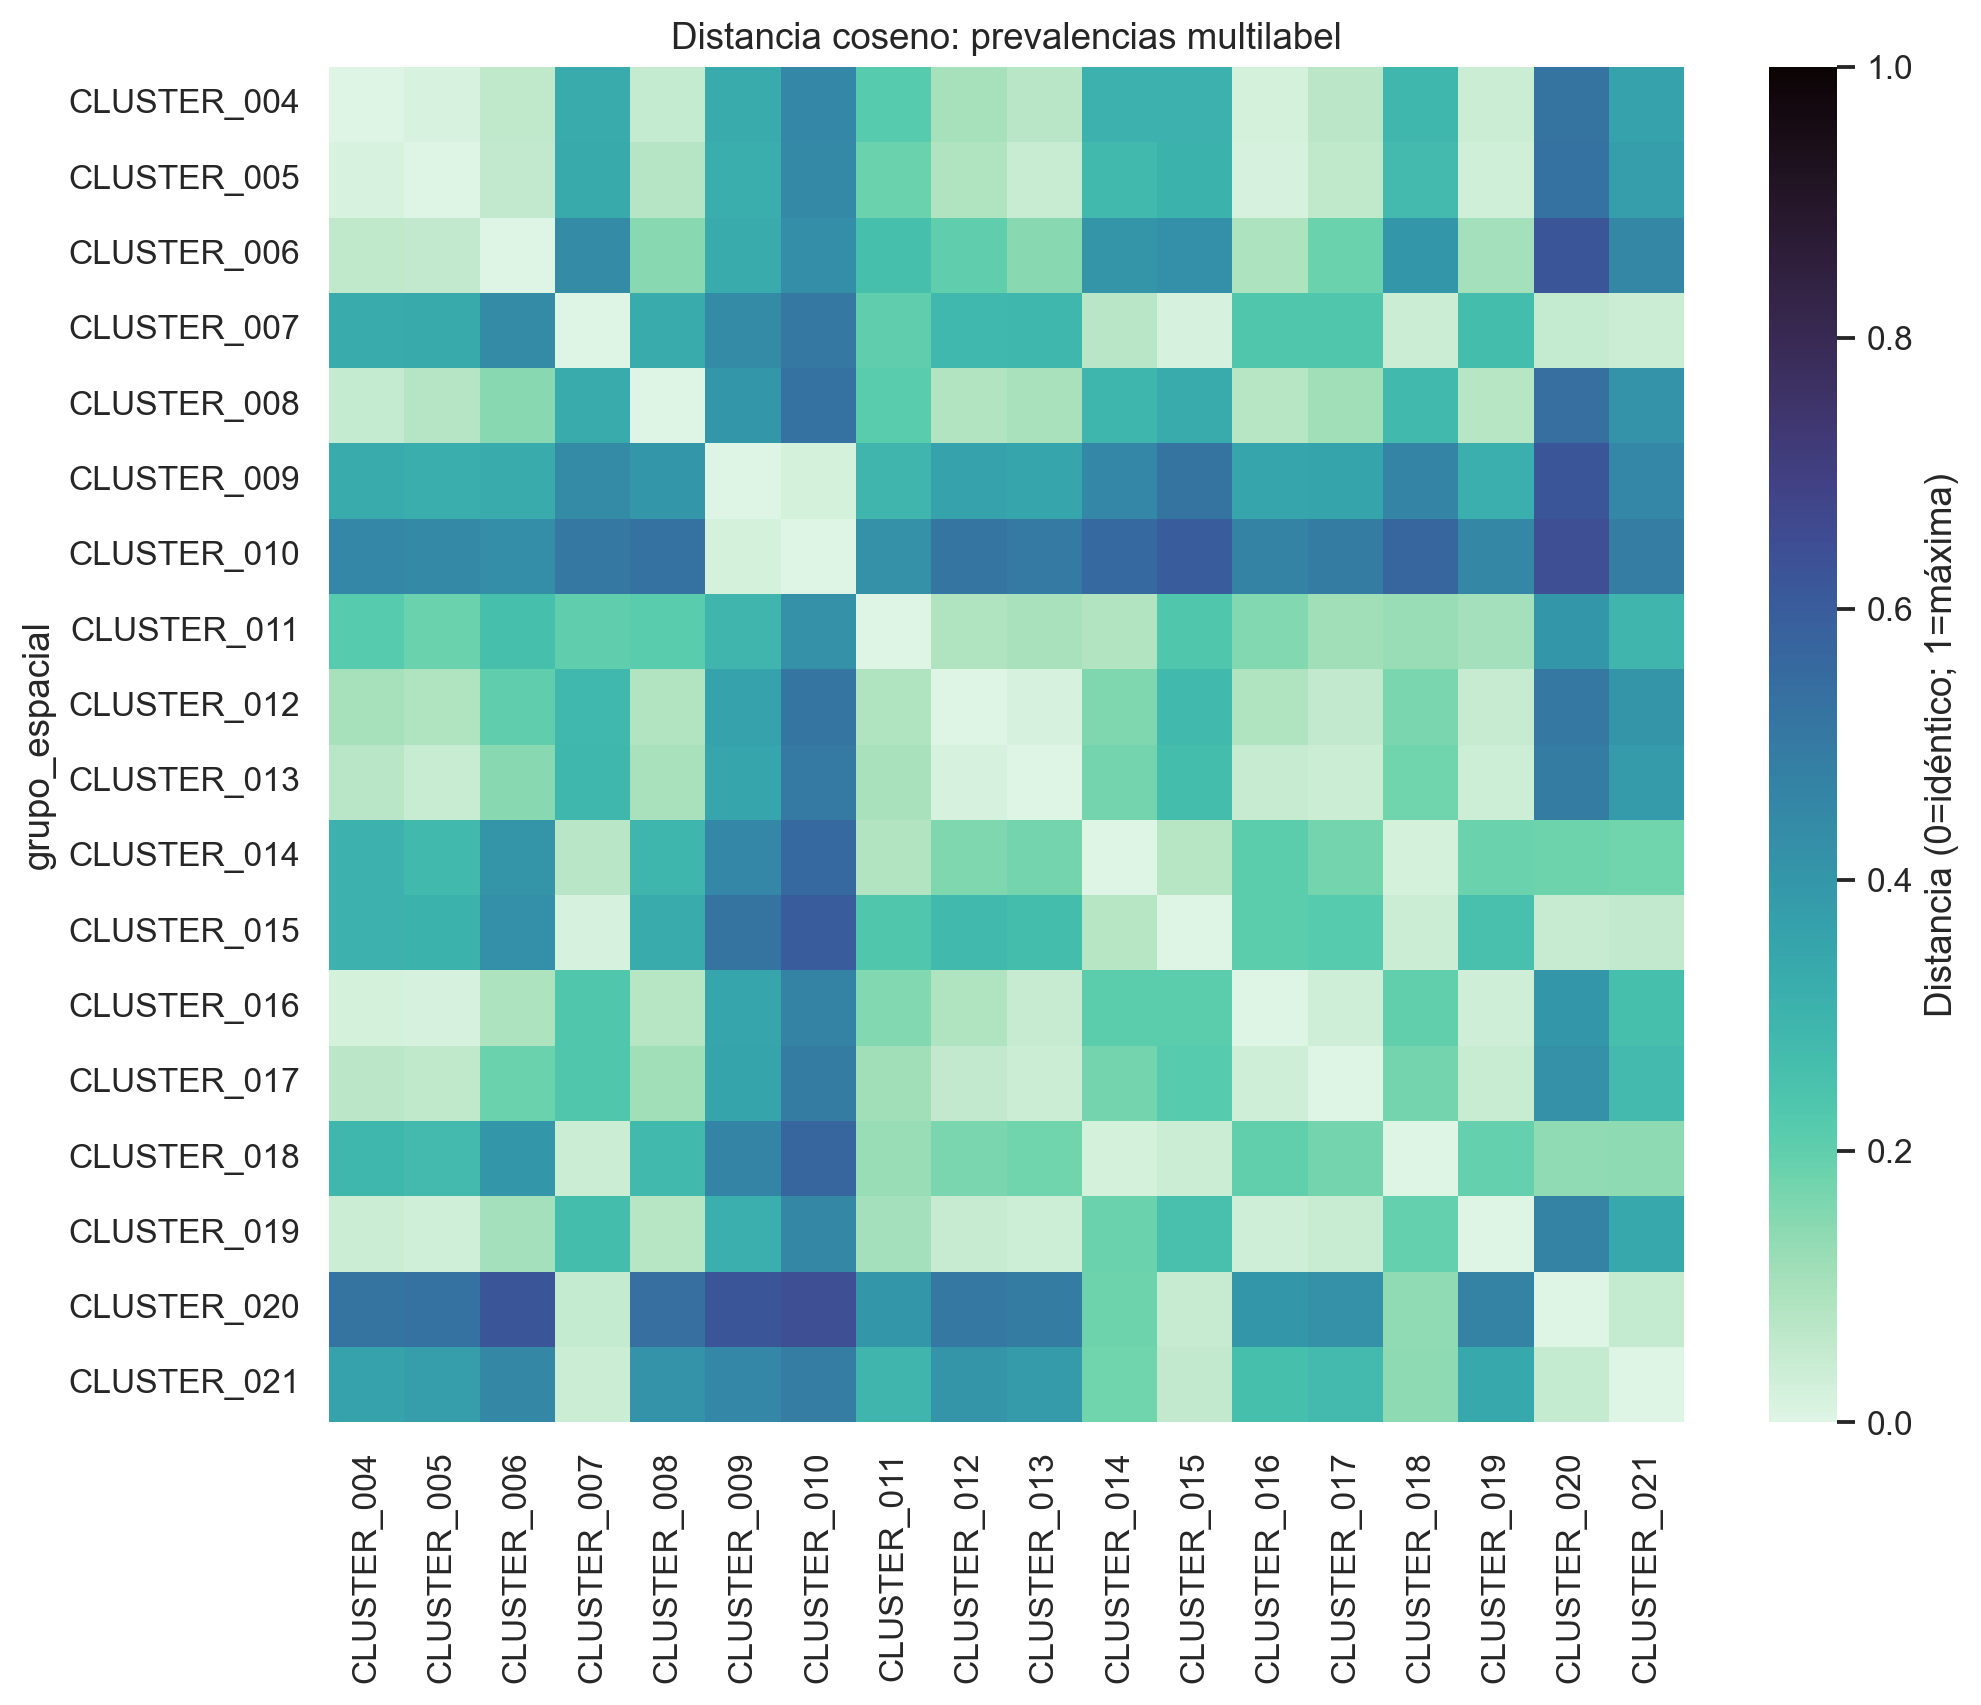
\includegraphics[width=.94\textwidth]{06_distancia_coseno_senales.png}\end{figure} \begin{figure}[H]\centering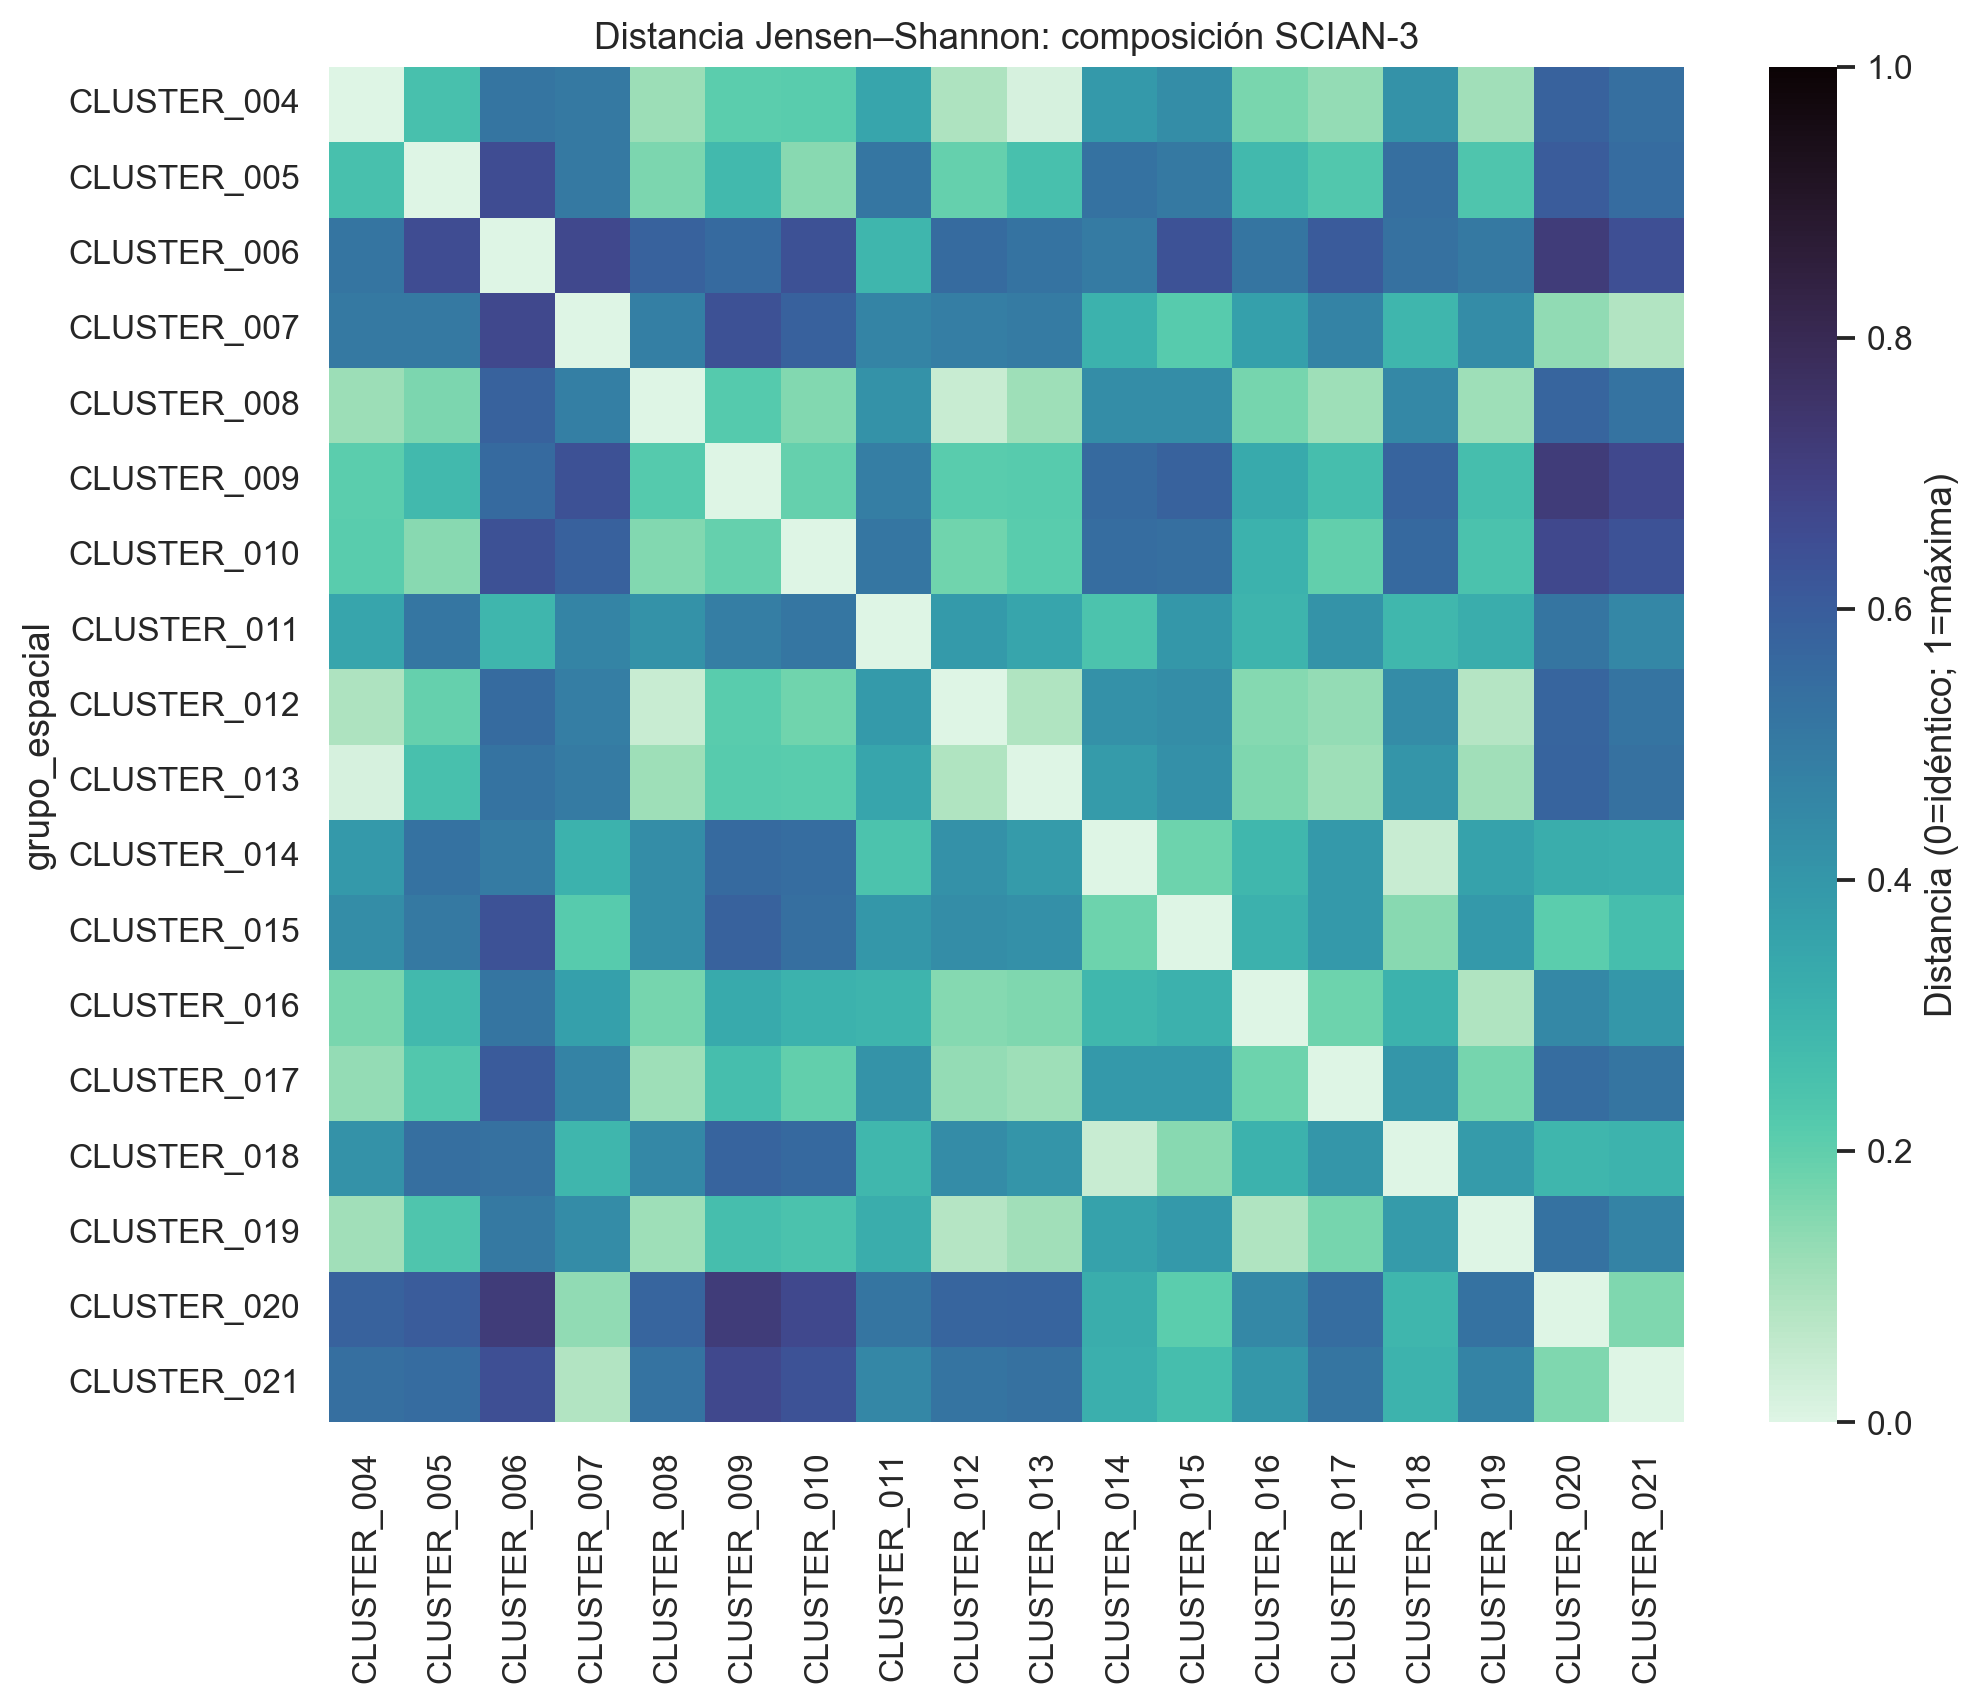
\includegraphics[width=.94\textwidth]{06_distancia_jensen_shannon_scian3.png}\end{figure} \begin{figure}[H]\centering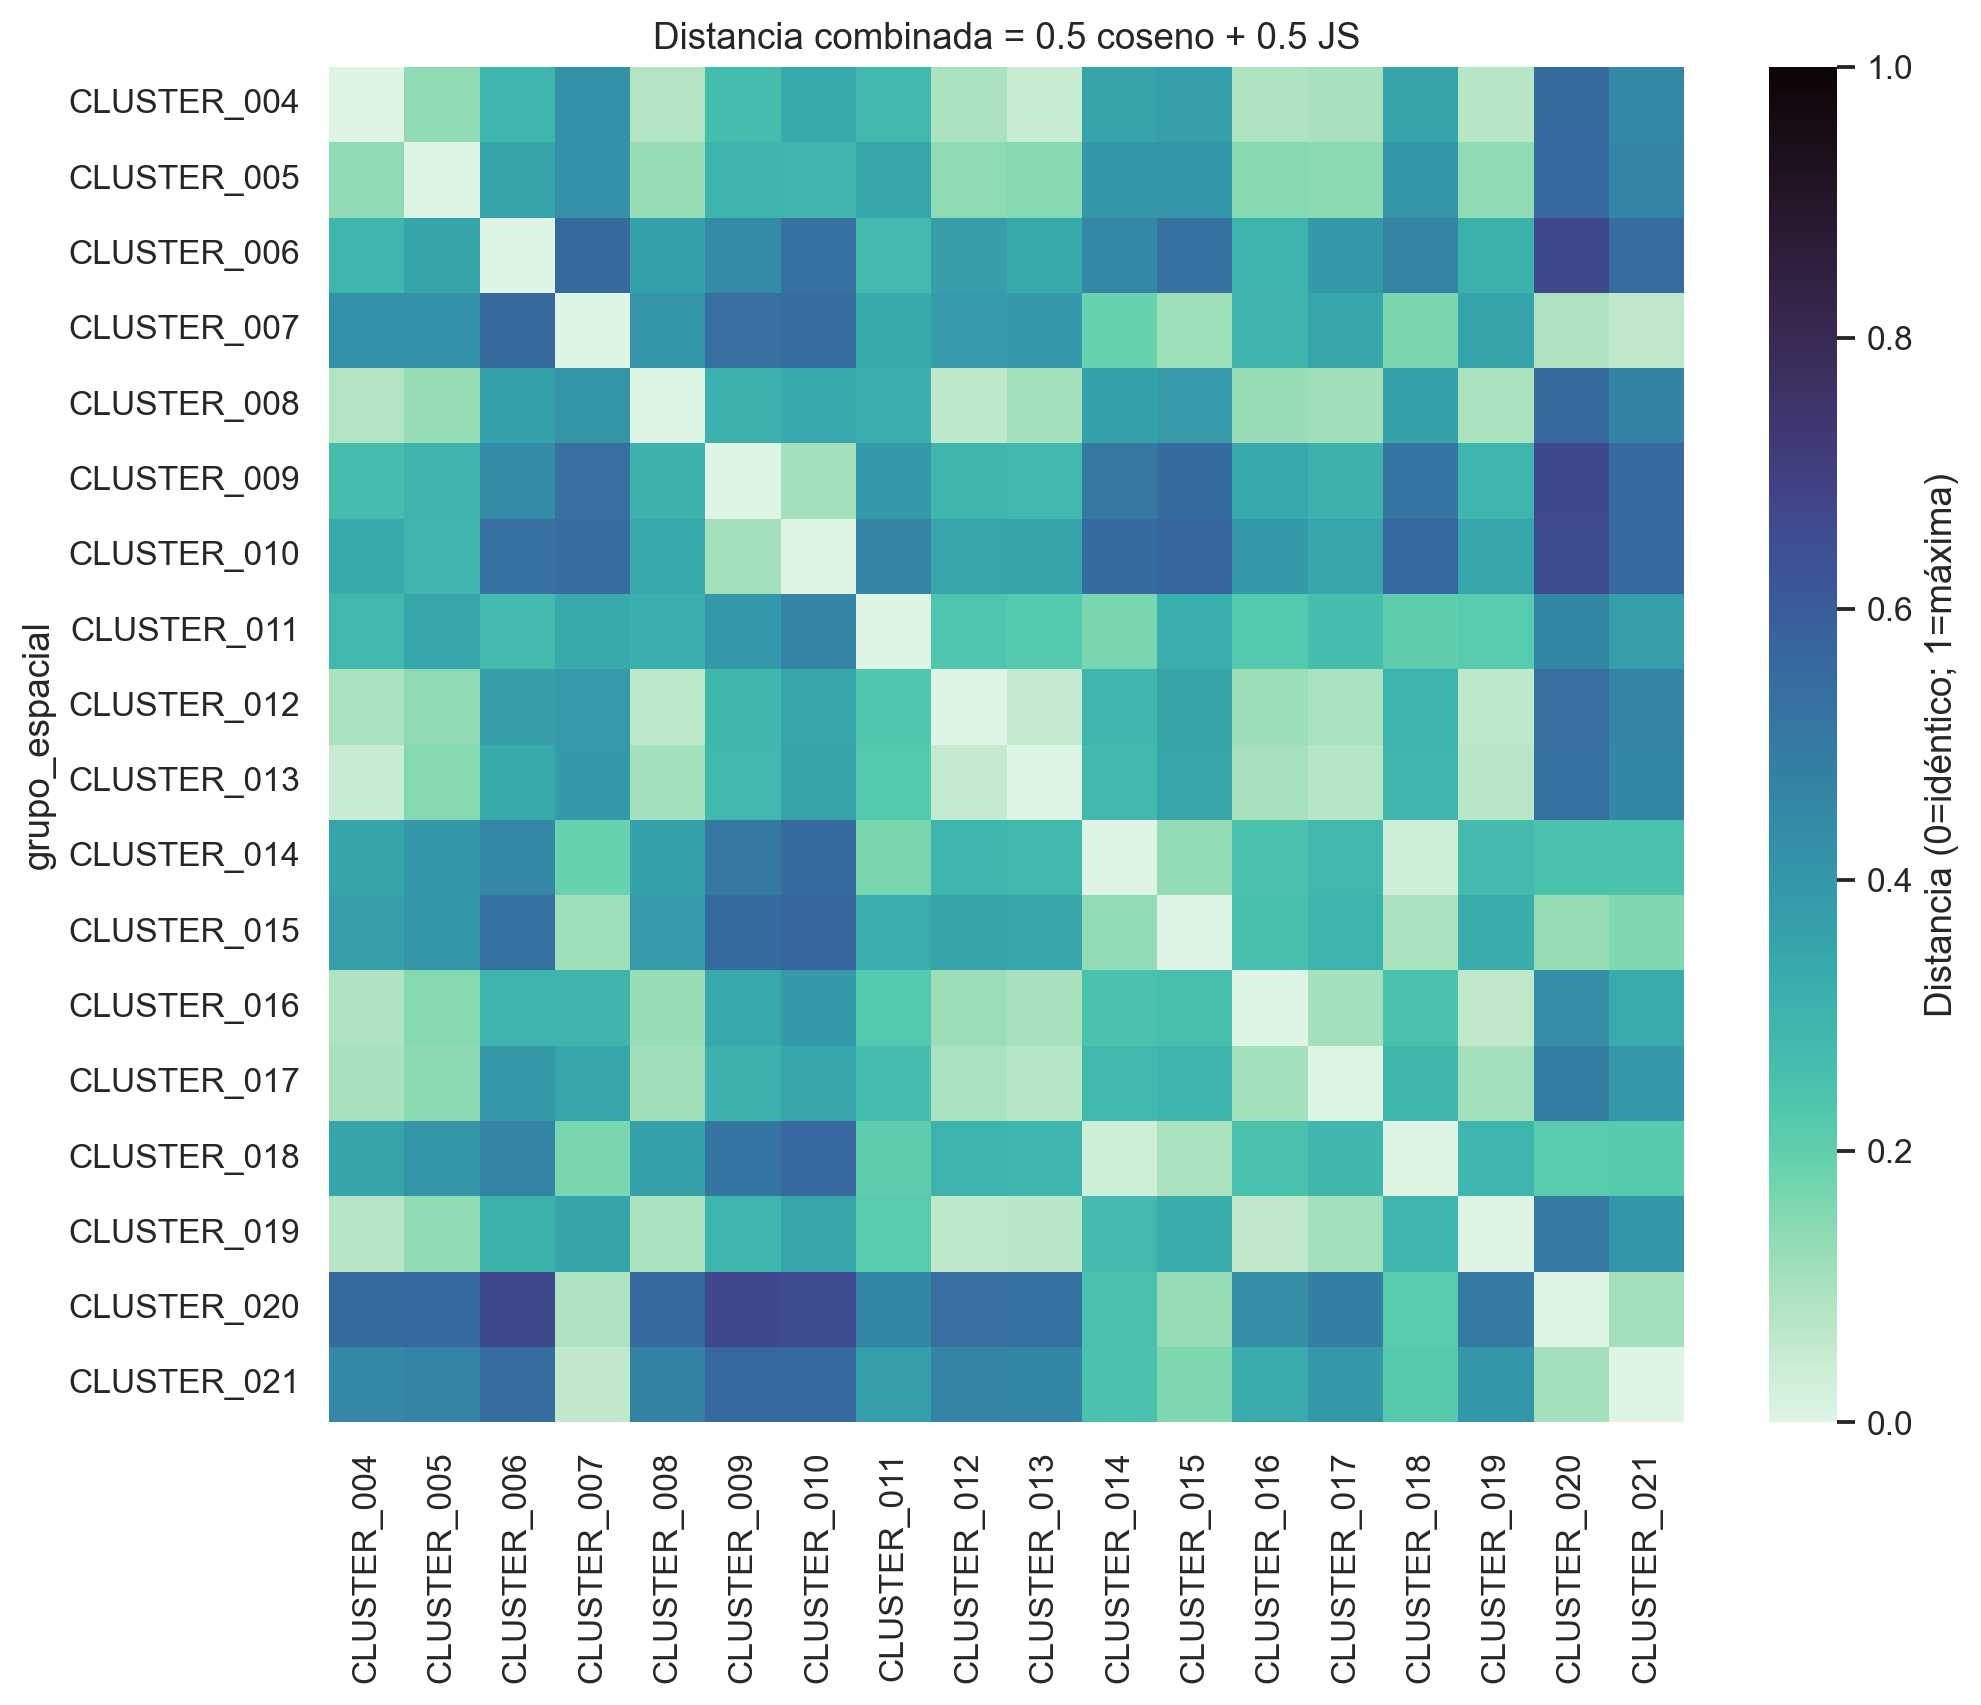
\includegraphics[width=.94\textwidth]{06_distancia_combinada_50_50.png}\end{figure} \begin{figure}[H]\centering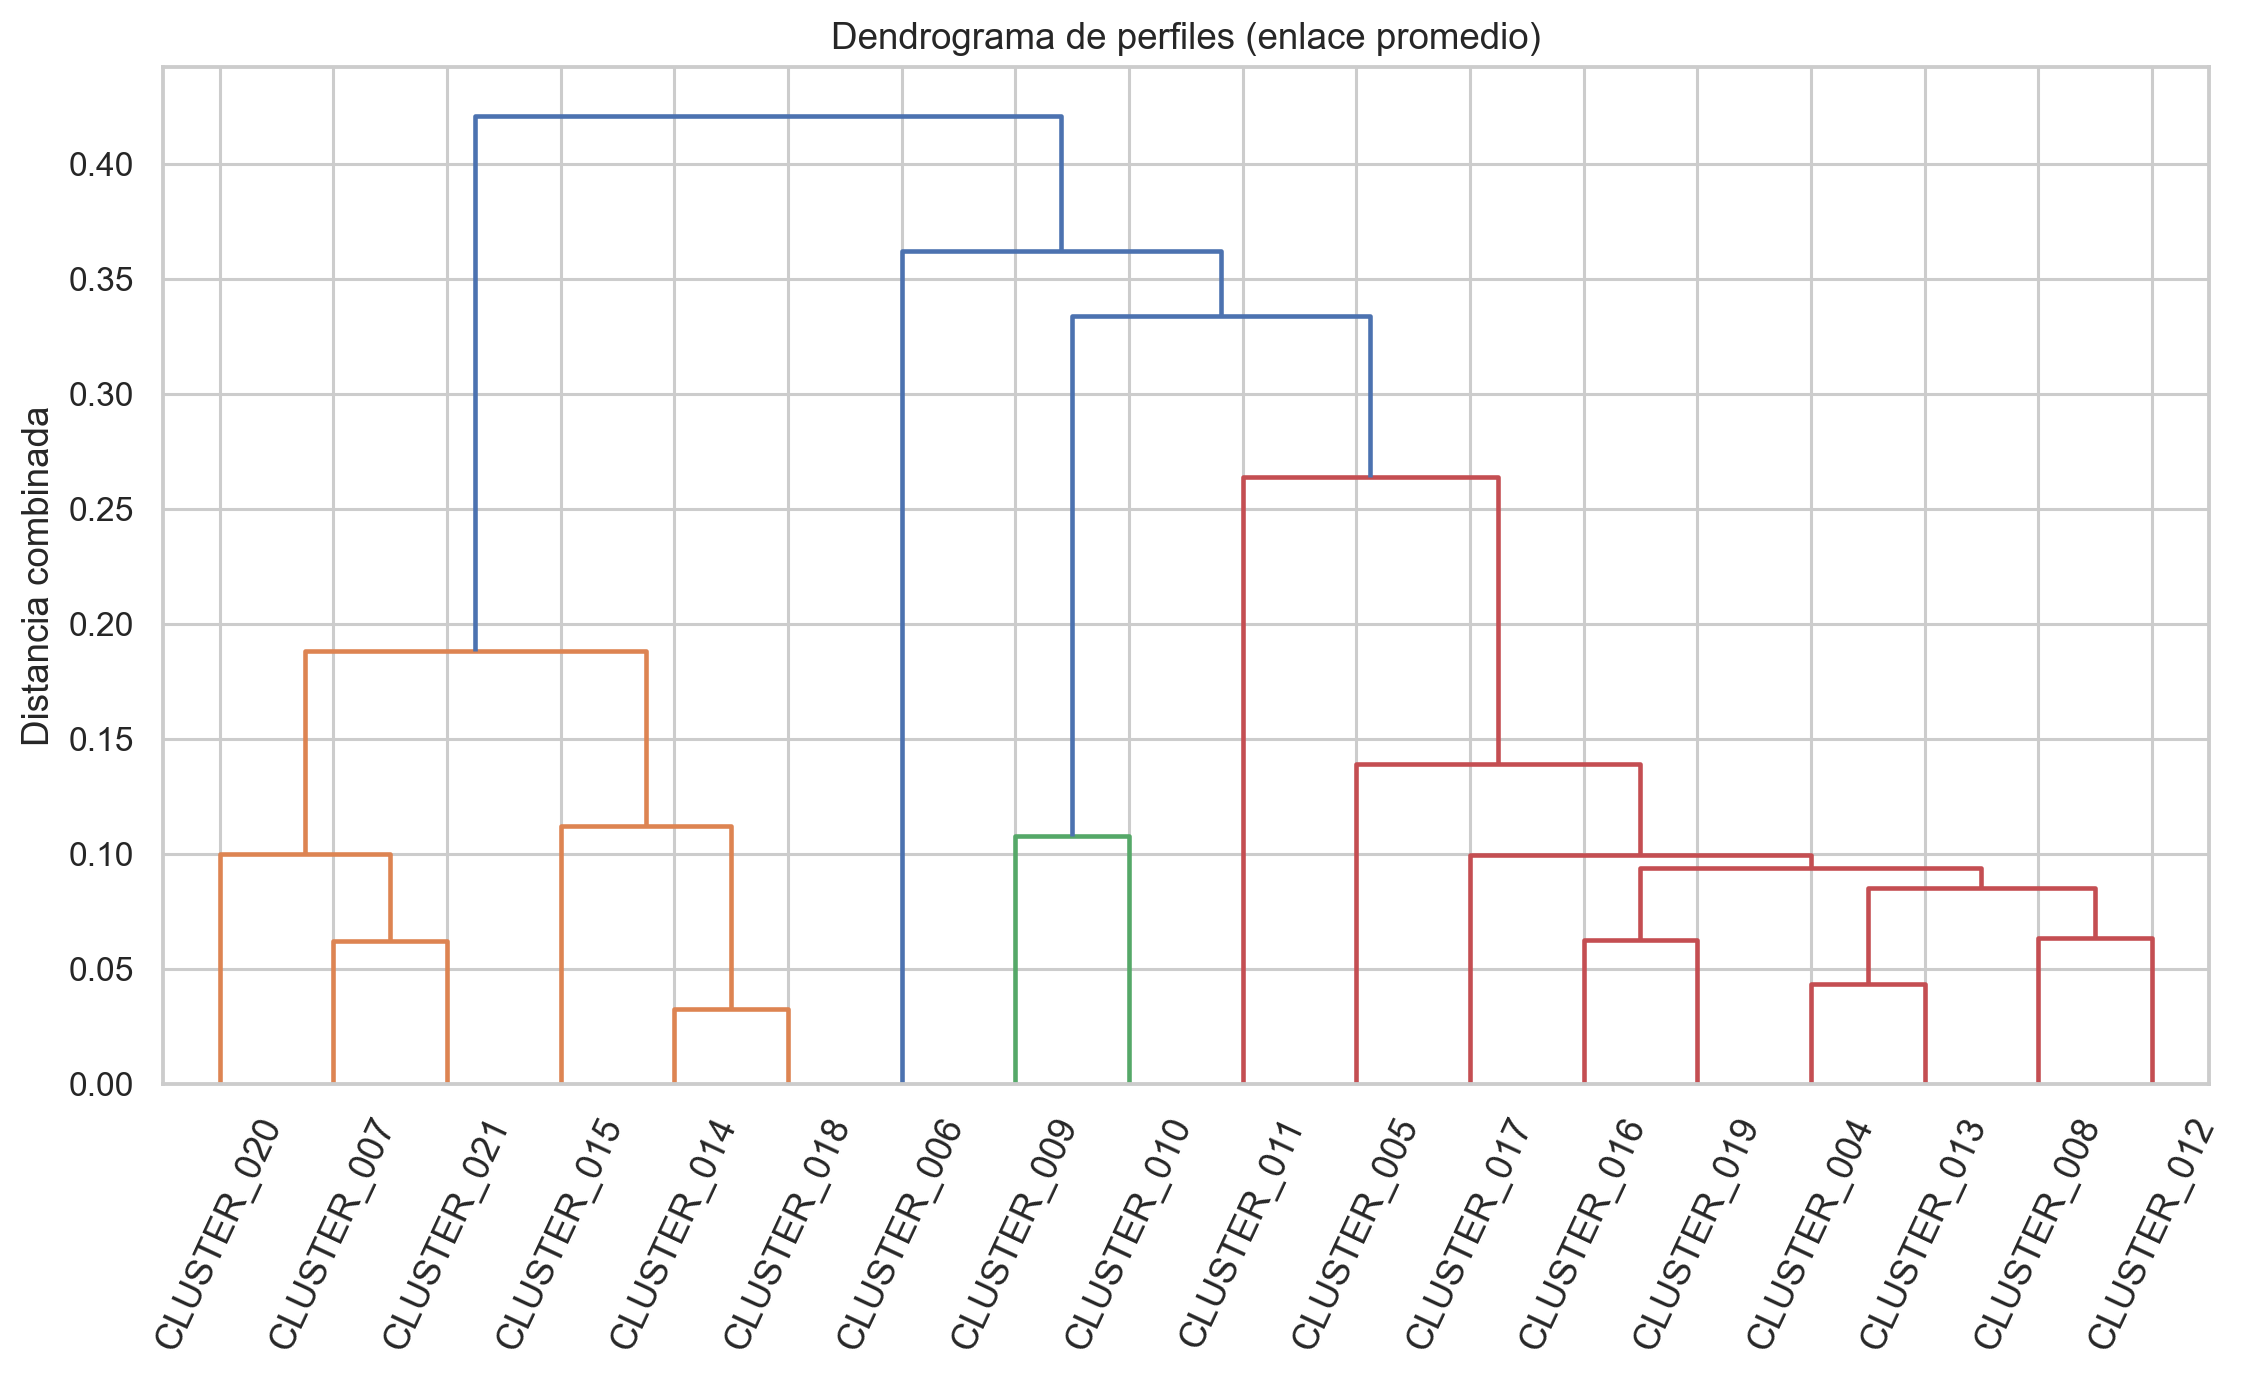
\includegraphics[width=.94\textwidth]{07_dendrograma_perfiles.png}\end{figure}\subsection{Por qué son similares los pares principales}{\scriptsize\setlength{\tabcolsep}{2pt}\begin{longtable}{>{\raggedright\arraybackslash}p{1.90cm}>{\raggedright\arraybackslash}p{1.90cm}>{\raggedright\arraybackslash}p{1.90cm}>{\raggedright\arraybackslash}p{1.90cm}>{\raggedright\arraybackslash}p{1.90cm}>{\raggedright\arraybackslash}p{1.90cm}>{\raggedright\arraybackslash}p{1.90cm}>{\raggedright\arraybackslash}p{1.90cm}}\toprule A & B & Cos. & JS & Comb. & Señales compartidas & SCIAN compartidos & Diferencias\\\midrule\endhead CLUSTER\_\allowbreak{}014 & CLUSTER\_\allowbreak{}018 & 0.021 & 0.045 & 0.033 & scian\_\allowbreak{}textil:59.4\% | textil:42.9\% | actividad\_\allowbreak{}confeccion:40.6\% | actividad\_\allowbreak{}lavanderia\_\allowbreak{}tintoreria:35.7\% | scian\_\allowbreak{}lavanderia:35.7\% & 315:40.6\% | 812:35.7\% | 314:18.8\% & proceso\_\allowbreak{}seco\_\allowbreak{}explicito:14.7pp | actividad\_\allowbreak{}bordado\_\allowbreak{}deshilado:12.1pp | produccion:9.8pp \\
CLUSTER\_\allowbreak{}004 & CLUSTER\_\allowbreak{}013 & 0.071 & 0.016 & 0.043 & scian\_\allowbreak{}textil:91.9\% | actividad\_\allowbreak{}confeccion:78.6\% | maquila:36.9\% | textil:28.6\% | scian\_\allowbreak{}lavanderia:7.1\% & 315:85.2\% | 812:7.1\% | 314:6.7\% & proceso\_\allowbreak{}seco\_\allowbreak{}explicito:40.5pp | textil:24.4pp | maquila:23.8pp \\
CLUSTER\_\allowbreak{}012 & CLUSTER\_\allowbreak{}013 & 0.017 & 0.089 & 0.053 & scian\_\allowbreak{}textil:91.9\% | actividad\_\allowbreak{}confeccion:81.2\% | textil:53.0\% | proceso\_\allowbreak{}seco\_\allowbreak{}explicito:47.7\% | maquila:25.0\% & 315:85.2\% | 812:7.1\% | 314:4.9\% & senal\_\allowbreak{}mezclilla\_\allowbreak{}o\_\allowbreak{}pantalon:13.8pp | textil:12.6pp | produccion:12.0pp \\
CLUSTER\_\allowbreak{}007 & CLUSTER\_\allowbreak{}021 & 0.040 & 0.084 & 0.062 & scian\_\allowbreak{}textil:55.6\% | scian\_\allowbreak{}lavanderia:41.9\% | actividad\_\allowbreak{}lavanderia\_\allowbreak{}tintoreria:41.9\% | lavado\_\allowbreak{}generico:37.4\% | actividad\_\allowbreak{}confeccion:25.8\% & 812:41.9\% | 315:29.0\% | 313:13.1\% & textil:21.0pp | proceso\_\allowbreak{}seco\_\allowbreak{}explicito:13.1pp | produccion:10.7pp \\
CLUSTER\_\allowbreak{}016 & CLUSTER\_\allowbreak{}019 & 0.035 & 0.090 & 0.062 & scian\_\allowbreak{}textil:84.3\% | actividad\_\allowbreak{}confeccion:70.6\% | maquila:44.0\% | textil:21.6\% | proceso\_\allowbreak{}seco\_\allowbreak{}explicito:17.6\% & 315:72.5\% | 314:9.0\% | 812:9.0\% & produccion:29.1pp | textil:17.4pp | lavado\_\allowbreak{}generico:7.7pp \\
CLUSTER\_\allowbreak{}008 & CLUSTER\_\allowbreak{}012 & 0.082 & 0.044 & 0.063 & scian\_\allowbreak{}textil:92.0\% | actividad\_\allowbreak{}confeccion:83.9\% | textil:45.1\% | maquila:25.0\% | proceso\_\allowbreak{}seco\_\allowbreak{}explicito:15.7\% & 315:86.6\% | 812:7.1\% | 314:3.0\% & proceso\_\allowbreak{}seco\_\allowbreak{}explicito:32.9pp | maquila:30.8pp | senal\_\allowbreak{}pantalon:27.4pp \\
CLUSTER\_\allowbreak{}012 & CLUSTER\_\allowbreak{}019 & 0.048 & 0.081 & 0.065 & scian\_\allowbreak{}textil:91.0\% | actividad\_\allowbreak{}confeccion:76.0\% | textil:39.0\% | maquila:25.0\% | proceso\_\allowbreak{}seco\_\allowbreak{}explicito:23.0\% & 315:80.0\% | 812:7.1\% | 314:4.9\% & textil:26.6pp | proceso\_\allowbreak{}seco\_\allowbreak{}explicito:25.7pp | maquila:19.0pp \\
CLUSTER\_\allowbreak{}013 & CLUSTER\_\allowbreak{}019 & 0.037 & 0.110 & 0.073 & scian\_\allowbreak{}textil:91.0\% | actividad\_\allowbreak{}confeccion:76.0\% | textil:39.0\% | maquila:36.9\% | proceso\_\allowbreak{}seco\_\allowbreak{}explicito:23.0\% & 315:80.0\% | 812:8.1\% | 314:6.7\% & produccion:25.6pp | proceso\_\allowbreak{}seco\_\allowbreak{}explicito:24.7pp | textil:14.0pp \\
CLUSTER\_\allowbreak{}004 & CLUSTER\_\allowbreak{}019 & 0.043 & 0.111 & 0.077 & scian\_\allowbreak{}textil:91.0\% | actividad\_\allowbreak{}confeccion:76.0\% | maquila:44.0\% | textil:28.6\% | scian\_\allowbreak{}lavanderia:7.1\% & 315:80.0\% | 314:7.1\% | 812:7.1\% & produccion:27.9pp | maquila:16.7pp | proceso\_\allowbreak{}seco\_\allowbreak{}explicito:15.9pp \\
CLUSTER\_\allowbreak{}013 & CLUSTER\_\allowbreak{}017 & 0.040 & 0.115 & 0.078 & scian\_\allowbreak{}textil:86.7\% | actividad\_\allowbreak{}confeccion:81.2\% | proceso\_\allowbreak{}seco\_\allowbreak{}explicito:24.4\% | textil:24.4\% | maquila:17.8\% & 315:84.4\% | 812:8.1\% | 314:2.2\% & textil:28.6pp | proceso\_\allowbreak{}seco\_\allowbreak{}explicito:23.2pp | maquila:19.1pp \\\bottomrule\end{longtable}}
\section{Explorador interactivo}\texttt{outputs/parte\_2/14\_segunda\_pasada/explorador\_interactivo\_clusters.html} es autocontenido: selecciona y compara dos clusters, ordena señales, alterna conteo/porcentaje, filtra señales presentes y cambia entre etiquetas compactas/ampliadas; muestra $n$, municipio, localidad, SCIAN, rasgos sobrerrepresentados, estabilidad, probabilidad y borde.
\section{Actividad dispersa, limitaciones y cierre}Los 578 puntos interiores no asignados son una categoría dependiente de escala, no un cluster equivalente. DENUE puede omitir actividad informal; la coordenada no prueba precisión predial; SCIAN 812210 no separa lavandería comercial de industrial; las etiquetas pueden correlacionarse. Concentración y coexistencia no prueban vínculos empresariales, consumo, descarga ni impacto. La relación hidrológica pertenece a Parte 3.

\section{Glosario metodológico permanente}
\small
\begin{longtable}{p{2.7cm}p{4.5cm}p{2.2cm}p{5.2cm}}\toprule Métrica & Definición/fórmula & Rango y lectura & Uso y advertencia\\\midrule\endhead
ARI & Acuerdo entre todos los pares de observaciones, corregido por azar: $(RI-E[RI])/(\max(RI)-E[RI])$. & 1 idéntico; cerca de 0 acuerdo esperable por azar; puede ser negativo. & Particiones completas; global, no identifica qué cluster cambia y puede estar dominado por grupos grandes.\\
Jaccard & $|A\cap B|/|A\cup B|$. & 0--1; alto indica mayor solapamiento. & Empareja clusters entre escenarios; no es estabilidad individual ni cohesión geométrica.\\
Estabilidad de membresía & $s_i=\frac1{5}\sum_k I[z_i^{(k)}=m_k(z_i)]$, donde $m_k$ es el cluster alternativo de máximo Jaccard. & 0--1; sensible 0--.49, estable .50--.79, núcleo robusto .80--1. & Cinco especificaciones, peso .2 cada una. No es persistencia nativa HDBSCAN.\\
Probabilidad HDBSCAN & Fuerza de pertenencia estimada por HDBSCAN respecto de la estructura de densidad. & 0--1; alta=membresía más fuerte. & No es probabilidad causal ni estabilidad entre modelos.\\
Persistencia HDBSCAN & Estabilidad de un cluster a través de niveles de densidad del árbol condensado. & No comparable directamente con $s_i$. & Sólo se informa cuando proviene de \texttt{cluster\_persistence\_}; no sustituye Jaccard.\\
Ruido & Etiqueta $-1$ para puntos no asignados a clusters bajo una especificación. & 0--100\%. & Depende de escala y parámetros; no significa irrelevancia.\\
Cluster mayor & $100\max_c n_c/N$. & 0--100\%. & Diagnóstico de dominancia, no error automático.\\
Densidad & $n/$área convexa en km$^2$. & $\ge0$; alta=más puntos por área. & Sensible a forma, borde y áreas casi nulas; no equivale a cohesión.\\
Prevalencia & $a/n$. & 0--1 o porcentaje. & Multilabel: columnas no suman 100\%.\\
Diferencia de prevalencias & $p_c-p_U$ (en tablas, puntos porcentuales). & $[-1,1]$. & Efecto absoluto descriptivo.\\
Lift / $\log_2$ lift & $p_c/p_U$; $\log_2(p_c/p_U)$. & Lift $>0$; log2=0 igualdad, $>0$ sobre-, $<0$ subrepresentación. & No implica causalidad; inestable con base rara.\\
Odds ratio e IC95 & $ad/(bc)$; IC con corrección Haldane--Anscombe de 0.5. & OR=1 sin asociación; IC que cruza 1 es compatible con nulo. & Comparación cluster/resto, no riesgo causal.\\
Fisher / BH & Prueba exacta 2x2; BH controla tasa esperada de falsos descubrimientos. & $p\in[0,1]$; filtro $p_{BH}\le.05$. & Significancia no sustituye tamaño de efecto.\\
Cosine similarity/distance & $s=(x\cdot y)/(\|x\|\|y\|)$; $d=1-s$. & En vectores no negativos, 0--1 para distancia. & Vector de 18 prevalencias; compara patrón, no volumen.\\
Jensen--Shannon divergence/distance & $JSD=\frac12 KL(P\|M)+\frac12 KL(Q\|M)$; distancia $\sqrt{JSD}$, base 2. & 0--1. & Distribuciones SCIAN a 3 dígitos normalizadas por cluster; se usa distancia de SciPy.\\
Distancia combinada & $d=.5d_{cos}+.5d_{JS}$. & 0--1; bajo=perfiles similares. & Pesos analíticos iguales; no usa geografía ni personal ocupado.\\
Centroide / medoide & Media de coordenadas / punto observado que minimiza suma de distancias. & Coordenadas métricas EPSG:32614. & Centroide puede no coincidir con un establecimiento; medoide sí.\\
KDE & Suma suavizada de kernels sobre puntos. & Intensidad relativa dependiente del ancho de banda. & Diagnóstico exploratorio; no define membresías.\\
Perturbación espacial & A cada coordenada se suma ruido independiente $N(0,25^2)$ m por eje y se reajusta el modelo. & 3 repeticiones, semilla 20260921. & Evalúa sensibilidad posicional local, no error geodésico completo.\\
\bottomrule\end{longtable}\normalsize
\appendix\section{Las 57 configuraciones exploradas}{\scriptsize\setlength{\tabcolsep}{2pt}\begin{longtable}{>{\raggedright\arraybackslash}p{2.17cm}>{\raggedright\arraybackslash}p{2.17cm}>{\raggedright\arraybackslash}p{2.17cm}>{\raggedright\arraybackslash}p{2.17cm}>{\raggedright\arraybackslash}p{2.17cm}>{\raggedright\arraybackslash}p{2.17cm}>{\raggedright\arraybackslash}p{2.17cm}}\toprule escenario\_\allowbreak{}id & metodo & n\_\allowbreak{}clusters & pct\_\allowbreak{}ruido & pct\_\allowbreak{}cluster\_\allowbreak{}mayor & ari\_\allowbreak{}top5\_\allowbreak{}mismo\_\allowbreak{}metodo & ari\_\allowbreak{}perturbacion\_\allowbreak{}25m\\\midrule\endhead hdbscan\_\allowbreak{}\_\allowbreak{}min\_\allowbreak{}cluster\_\allowbreak{}size-30\_\allowbreak{}\_\allowbreak{}min\_\allowbreak{}samples-5\_\allowbreak{}\_\allowbreak{}cluster\_\allowbreak{}selection\_\allowbreak{}method-eom & HDBSCAN & 19 & 6.117 & 52.921 & 0.928 & 0.942 \\
dbscan\_\allowbreak{}\_\allowbreak{}eps\_\allowbreak{}m-1200\_\allowbreak{}\_\allowbreak{}min\_\allowbreak{}samples-10 & DBSCAN & 24 & 3.276 & 50.790 & 0.950 & 0.999 \\
dbscan\_\allowbreak{}\_\allowbreak{}eps\_\allowbreak{}m-800\_\allowbreak{}\_\allowbreak{}min\_\allowbreak{}samples-10 & DBSCAN & 25 & 8.683 & 46.575 & 0.915 & 0.996 \\
dbscan\_\allowbreak{}\_\allowbreak{}eps\_\allowbreak{}m-1200\_\allowbreak{}\_\allowbreak{}min\_\allowbreak{}samples-25 & DBSCAN & 13 & 11.684 & 46.964 & 0.910 & 0.979 \\
dbscan\_\allowbreak{}\_\allowbreak{}eps\_\allowbreak{}m-1200\_\allowbreak{}\_\allowbreak{}min\_\allowbreak{}samples-15 & DBSCAN & 20 & 6.300 & 48.866 & 0.929 & 0.991 \\
dbscan\_\allowbreak{}\_\allowbreak{}eps\_\allowbreak{}m-1600\_\allowbreak{}\_\allowbreak{}min\_\allowbreak{}samples-15 & DBSCAN & 17 & 3.322 & 51.409 & 0.945 & 0.978 \\
dbscan\_\allowbreak{}\_\allowbreak{}eps\_\allowbreak{}m-600\_\allowbreak{}\_\allowbreak{}min\_\allowbreak{}samples-5 & DBSCAN & 51 & 5.361 & 45.750 & 0.896 & 0.984 \\
dbscan\_\allowbreak{}\_\allowbreak{}eps\_\allowbreak{}m-1200\_\allowbreak{}\_\allowbreak{}min\_\allowbreak{}samples-5 & DBSCAN & 27 & 1.168 & 53.081 & 0.932 & 1.000 \\
dbscan\_\allowbreak{}\_\allowbreak{}eps\_\allowbreak{}m-800\_\allowbreak{}\_\allowbreak{}min\_\allowbreak{}samples-5 & DBSCAN & 44 & 2.428 & 49.255 & 0.916 & 0.989 \\
dbscan\_\allowbreak{}\_\allowbreak{}eps\_\allowbreak{}m-1600\_\allowbreak{}\_\allowbreak{}min\_\allowbreak{}samples-10 & DBSCAN & 16 & 1.856 & 55.785 & 0.907 & 0.998 \\
dbscan\_\allowbreak{}\_\allowbreak{}eps\_\allowbreak{}m-1600\_\allowbreak{}\_\allowbreak{}min\_\allowbreak{}samples-5 & DBSCAN & 22 & 0.619 & 56.403 & 0.896 & 1.000 \\
hdbscan\_\allowbreak{}\_\allowbreak{}min\_\allowbreak{}cluster\_\allowbreak{}size-75\_\allowbreak{}\_\allowbreak{}min\_\allowbreak{}samples-10\_\allowbreak{}\_\allowbreak{}cluster\_\allowbreak{}selection\_\allowbreak{}method-eom & HDBSCAN & 9 & 9.576 & 51.226 & 0.944 & 0.994 \\
hdbscan\_\allowbreak{}\_\allowbreak{}min\_\allowbreak{}cluster\_\allowbreak{}size-75\_\allowbreak{}\_\allowbreak{}min\_\allowbreak{}samples-20\_\allowbreak{}\_\allowbreak{}cluster\_\allowbreak{}selection\_\allowbreak{}method-eom & HDBSCAN & 9 & 11.959 & 49.301 & 0.921 & 0.980 \\
dbscan\_\allowbreak{}\_\allowbreak{}eps\_\allowbreak{}m-800\_\allowbreak{}\_\allowbreak{}min\_\allowbreak{}samples-15 & DBSCAN & 25 & 12.234 & 38.007 & 0.732 & 0.976 \\
hdbscan\_\allowbreak{}\_\allowbreak{}min\_\allowbreak{}cluster\_\allowbreak{}size-50\_\allowbreak{}\_\allowbreak{}min\_\allowbreak{}samples-20\_\allowbreak{}\_\allowbreak{}cluster\_\allowbreak{}selection\_\allowbreak{}method-eom & HDBSCAN & 10 & 10.745 & 49.301 & 0.923 & 0.981 \\
hdbscan\_\allowbreak{}\_\allowbreak{}min\_\allowbreak{}cluster\_\allowbreak{}size-75\_\allowbreak{}\_\allowbreak{}min\_\allowbreak{}samples-5\_\allowbreak{}\_\allowbreak{}cluster\_\allowbreak{}selection\_\allowbreak{}method-eom & HDBSCAN & 9 & 6.964 & 52.921 & 0.942 & 0.999 \\
hdbscan\_\allowbreak{}\_\allowbreak{}min\_\allowbreak{}cluster\_\allowbreak{}size-50\_\allowbreak{}\_\allowbreak{}min\_\allowbreak{}samples-10\_\allowbreak{}\_\allowbreak{}cluster\_\allowbreak{}selection\_\allowbreak{}method-eom & HDBSCAN & 13 & 8.408 & 51.226 & 0.932 & 0.979 \\
hdbscan\_\allowbreak{}\_\allowbreak{}min\_\allowbreak{}cluster\_\allowbreak{}size-50\_\allowbreak{}\_\allowbreak{}min\_\allowbreak{}samples-5\_\allowbreak{}\_\allowbreak{}cluster\_\allowbreak{}selection\_\allowbreak{}method-eom & HDBSCAN & 10 & 5.750 & 52.921 & 0.943 & 0.999 \\
dbscan\_\allowbreak{}\_\allowbreak{}eps\_\allowbreak{}m-600\_\allowbreak{}\_\allowbreak{}min\_\allowbreak{}samples-15 & DBSCAN & 34 & 25.727 & 22.451 & 0.602 & 0.902 \\
dbscan\_\allowbreak{}\_\allowbreak{}eps\_\allowbreak{}m-800\_\allowbreak{}\_\allowbreak{}min\_\allowbreak{}samples-25 & DBSCAN & 23 & 27.858 & 22.199 & 0.575 & 0.968 \\
hdbscan\_\allowbreak{}\_\allowbreak{}min\_\allowbreak{}cluster\_\allowbreak{}size-20\_\allowbreak{}\_\allowbreak{}min\_\allowbreak{}samples-20\_\allowbreak{}\_\allowbreak{}cluster\_\allowbreak{}selection\_\allowbreak{}method-leaf & HDBSCAN & 40 & 51.019 & 5.132 & 0.659 & 0.818 \\
hdbscan\_\allowbreak{}\_\allowbreak{}min\_\allowbreak{}cluster\_\allowbreak{}size-30\_\allowbreak{}\_\allowbreak{}min\_\allowbreak{}samples-20\_\allowbreak{}\_\allowbreak{}cluster\_\allowbreak{}selection\_\allowbreak{}method-leaf & HDBSCAN & 34 & 51.088 & 5.132 & 0.651 & 0.813 \\
dbscan\_\allowbreak{}\_\allowbreak{}eps\_\allowbreak{}m-600\_\allowbreak{}\_\allowbreak{}min\_\allowbreak{}samples-10 & DBSCAN & 40 & 13.356 & 27.491 & 0.612 & 0.922 \\
hdbscan\_\allowbreak{}\_\allowbreak{}min\_\allowbreak{}cluster\_\allowbreak{}size-20\_\allowbreak{}\_\allowbreak{}min\_\allowbreak{}samples-10\_\allowbreak{}\_\allowbreak{}cluster\_\allowbreak{}selection\_\allowbreak{}method-leaf & HDBSCAN & 57 & 43.184 & 2.566 & 0.622 & 0.765 \\
hdbscan\_\allowbreak{}\_\allowbreak{}min\_\allowbreak{}cluster\_\allowbreak{}size-30\_\allowbreak{}\_\allowbreak{}min\_\allowbreak{}samples-10\_\allowbreak{}\_\allowbreak{}cluster\_\allowbreak{}selection\_\allowbreak{}method-leaf & HDBSCAN & 42 & 41.581 & 2.566 & 0.615 & 0.765 \\
dbscan\_\allowbreak{}\_\allowbreak{}eps\_\allowbreak{}m-400\_\allowbreak{}\_\allowbreak{}min\_\allowbreak{}samples-25 & DBSCAN & 12 & 71.775 & 7.652 & 0.709 & 0.970 \\
dbscan\_\allowbreak{}\_\allowbreak{}eps\_\allowbreak{}m-250\_\allowbreak{}\_\allowbreak{}min\_\allowbreak{}samples-10 & DBSCAN & 31 & 66.071 & 7.491 & 0.698 & 0.921 \\
dbscan\_\allowbreak{}\_\allowbreak{}eps\_\allowbreak{}m-250\_\allowbreak{}\_\allowbreak{}min\_\allowbreak{}samples-15 & DBSCAN & 14 & 74.044 & 7.331 & 0.696 & 0.959 \\
dbscan\_\allowbreak{}\_\allowbreak{}eps\_\allowbreak{}m-400\_\allowbreak{}\_\allowbreak{}min\_\allowbreak{}samples-15 & DBSCAN & 29 & 58.190 & 7.675 & 0.643 & 0.927 \\
hdbscan\_\allowbreak{}\_\allowbreak{}min\_\allowbreak{}cluster\_\allowbreak{}size-30\_\allowbreak{}\_\allowbreak{}min\_\allowbreak{}samples-5\_\allowbreak{}\_\allowbreak{}cluster\_\allowbreak{}selection\_\allowbreak{}method-leaf & HDBSCAN & 47 & 32.692 & 3.024 & 0.557 & 0.680 \\
hdbscan\_\allowbreak{}\_\allowbreak{}min\_\allowbreak{}cluster\_\allowbreak{}size-10\_\allowbreak{}\_\allowbreak{}min\_\allowbreak{}samples-20\_\allowbreak{}\_\allowbreak{}cluster\_\allowbreak{}selection\_\allowbreak{}method-leaf & HDBSCAN & 53 & 55.281 & 2.291 & 0.590 & 0.839 \\
dbscan\_\allowbreak{}\_\allowbreak{}eps\_\allowbreak{}m-600\_\allowbreak{}\_\allowbreak{}min\_\allowbreak{}samples-25 & DBSCAN & 27 & 52.027 & 7.698 & 0.574 & 0.953 \\
dbscan\_\allowbreak{}\_\allowbreak{}eps\_\allowbreak{}m-400\_\allowbreak{}\_\allowbreak{}min\_\allowbreak{}samples-10 & DBSCAN & 69 & 36.724 & 7.698 & 0.534 & 0.877 \\
hdbscan\_\allowbreak{}\_\allowbreak{}min\_\allowbreak{}cluster\_\allowbreak{}size-20\_\allowbreak{}\_\allowbreak{}min\_\allowbreak{}samples-5\_\allowbreak{}\_\allowbreak{}cluster\_\allowbreak{}selection\_\allowbreak{}method-leaf & HDBSCAN & 70 & 33.906 & 2.360 & 0.525 & 0.649 \\
hdbscan\_\allowbreak{}\_\allowbreak{}min\_\allowbreak{}cluster\_\allowbreak{}size-10\_\allowbreak{}\_\allowbreak{}min\_\allowbreak{}samples-5\_\allowbreak{}\_\allowbreak{}cluster\_\allowbreak{}selection\_\allowbreak{}method-eom & HDBSCAN & 99 & 21.879 & 7.789 & 0.479 & 0.762 \\
hdbscan\_\allowbreak{}\_\allowbreak{}min\_\allowbreak{}cluster\_\allowbreak{}size-50\_\allowbreak{}\_\allowbreak{}min\_\allowbreak{}samples-20\_\allowbreak{}\_\allowbreak{}cluster\_\allowbreak{}selection\_\allowbreak{}method-leaf & HDBSCAN & 19 & 45.590 & 7.721 & 0.664 & 0.909 \\
hdbscan\_\allowbreak{}\_\allowbreak{}min\_\allowbreak{}cluster\_\allowbreak{}size-10\_\allowbreak{}\_\allowbreak{}min\_\allowbreak{}samples-10\_\allowbreak{}\_\allowbreak{}cluster\_\allowbreak{}selection\_\allowbreak{}method-eom & HDBSCAN & 73 & 29.187 & 7.721 & 0.487 & 0.609 \\
hdbscan\_\allowbreak{}\_\allowbreak{}min\_\allowbreak{}cluster\_\allowbreak{}size-20\_\allowbreak{}\_\allowbreak{}min\_\allowbreak{}samples-5\_\allowbreak{}\_\allowbreak{}cluster\_\allowbreak{}selection\_\allowbreak{}method-eom & HDBSCAN & 55 & 22.108 & 7.789 & 0.525 & 0.388 \\
hdbscan\_\allowbreak{}\_\allowbreak{}min\_\allowbreak{}cluster\_\allowbreak{}size-75\_\allowbreak{}\_\allowbreak{}min\_\allowbreak{}samples-10\_\allowbreak{}\_\allowbreak{}cluster\_\allowbreak{}selection\_\allowbreak{}method-leaf & HDBSCAN & 18 & 40.802 & 7.721 & 0.616 & 0.854 \\
hdbscan\_\allowbreak{}\_\allowbreak{}min\_\allowbreak{}cluster\_\allowbreak{}size-75\_\allowbreak{}\_\allowbreak{}min\_\allowbreak{}samples-20\_\allowbreak{}\_\allowbreak{}cluster\_\allowbreak{}selection\_\allowbreak{}method-leaf & HDBSCAN & 15 & 50.584 & 7.721 & 0.633 & 0.908 \\
dbscan\_\allowbreak{}\_\allowbreak{}eps\_\allowbreak{}m-400\_\allowbreak{}\_\allowbreak{}min\_\allowbreak{}samples-5 & DBSCAN & 91 & 14.502 & 16.655 & 0.479 & 0.801 \\
hdbscan\_\allowbreak{}\_\allowbreak{}min\_\allowbreak{}cluster\_\allowbreak{}size-10\_\allowbreak{}\_\allowbreak{}min\_\allowbreak{}samples-10\_\allowbreak{}\_\allowbreak{}cluster\_\allowbreak{}selection\_\allowbreak{}method-leaf & HDBSCAN & 94 & 45.109 & 2.131 & 0.505 & 0.701 \\
dbscan\_\allowbreak{}\_\allowbreak{}eps\_\allowbreak{}m-250\_\allowbreak{}\_\allowbreak{}min\_\allowbreak{}samples-25 & DBSCAN & 8 & 81.672 & 5.773 & 0.542 & 0.952 \\
hdbscan\_\allowbreak{}\_\allowbreak{}min\_\allowbreak{}cluster\_\allowbreak{}size-75\_\allowbreak{}\_\allowbreak{}min\_\allowbreak{}samples-5\_\allowbreak{}\_\allowbreak{}cluster\_\allowbreak{}selection\_\allowbreak{}method-leaf & HDBSCAN & 17 & 44.536 & 7.789 & 0.573 & 0.778 \\
hdbscan\_\allowbreak{}\_\allowbreak{}min\_\allowbreak{}cluster\_\allowbreak{}size-50\_\allowbreak{}\_\allowbreak{}min\_\allowbreak{}samples-10\_\allowbreak{}\_\allowbreak{}cluster\_\allowbreak{}selection\_\allowbreak{}method-leaf & HDBSCAN & 27 & 41.764 & 4.834 & 0.577 & 0.721 \\
hdbscan\_\allowbreak{}\_\allowbreak{}min\_\allowbreak{}cluster\_\allowbreak{}size-50\_\allowbreak{}\_\allowbreak{}min\_\allowbreak{}samples-5\_\allowbreak{}\_\allowbreak{}cluster\_\allowbreak{}selection\_\allowbreak{}method-leaf & HDBSCAN & 29 & 38.877 & 5.109 & 0.524 & 0.710 \\
hdbscan\_\allowbreak{}\_\allowbreak{}min\_\allowbreak{}cluster\_\allowbreak{}size-10\_\allowbreak{}\_\allowbreak{}min\_\allowbreak{}samples-5\_\allowbreak{}\_\allowbreak{}cluster\_\allowbreak{}selection\_\allowbreak{}method-leaf & HDBSCAN & 134 & 32.875 & 1.787 & 0.439 & 0.624 \\
dbscan\_\allowbreak{}\_\allowbreak{}eps\_\allowbreak{}m-250\_\allowbreak{}\_\allowbreak{}min\_\allowbreak{}samples-5 & DBSCAN & 149 & 39.038 & 7.606 & 0.463 & 0.852 \\
optics\_\allowbreak{}\_\allowbreak{}min\_\allowbreak{}samples-20\_\allowbreak{}\_\allowbreak{}xi-0p05\_\allowbreak{}\_\allowbreak{}min\_\allowbreak{}cluster\_\allowbreak{}size\_\allowbreak{}frac-0p01 & OPTICS & 21 & 62.085 & 7.789 & 0.560 & nan \\
optics\_\allowbreak{}\_\allowbreak{}min\_\allowbreak{}samples-30\_\allowbreak{}\_\allowbreak{}xi-0p05\_\allowbreak{}\_\allowbreak{}min\_\allowbreak{}cluster\_\allowbreak{}size\_\allowbreak{}frac-0p01 & OPTICS & 18 & 61.512 & 7.789 & 0.531 & nan \\
optics\_\allowbreak{}\_\allowbreak{}min\_\allowbreak{}samples-10\_\allowbreak{}\_\allowbreak{}xi-0p05\_\allowbreak{}\_\allowbreak{}min\_\allowbreak{}cluster\_\allowbreak{}size\_\allowbreak{}frac-0p01 & OPTICS & 28 & 60.206 & 2.131 & 0.415 & nan \\
hdbscan\_\allowbreak{}\_\allowbreak{}min\_\allowbreak{}cluster\_\allowbreak{}size-10\_\allowbreak{}\_\allowbreak{}min\_\allowbreak{}samples-20\_\allowbreak{}\_\allowbreak{}cluster\_\allowbreak{}selection\_\allowbreak{}method-eom & HDBSCAN & 22 & 13.379 & 45.750 & 0.937 & 0.926 \\
dbscan\_\allowbreak{}\_\allowbreak{}eps\_\allowbreak{}m-1600\_\allowbreak{}\_\allowbreak{}min\_\allowbreak{}samples-25 & DBSCAN & 13 & 7.537 & 49.897 & 0.933 & 0.996 \\
hdbscan\_\allowbreak{}\_\allowbreak{}min\_\allowbreak{}cluster\_\allowbreak{}size-20\_\allowbreak{}\_\allowbreak{}min\_\allowbreak{}samples-20\_\allowbreak{}\_\allowbreak{}cluster\_\allowbreak{}selection\_\allowbreak{}method-eom & HDBSCAN & 21 & 13.700 & 45.750 & 0.936 & 0.926 \\
hdbscan\_\allowbreak{}\_\allowbreak{}min\_\allowbreak{}cluster\_\allowbreak{}size-30\_\allowbreak{}\_\allowbreak{}min\_\allowbreak{}samples-20\_\allowbreak{}\_\allowbreak{}cluster\_\allowbreak{}selection\_\allowbreak{}method-eom & HDBSCAN & 18 & 14.800 & 45.750 & 0.933 & 0.921 \\
hdbscan\_\allowbreak{}\_\allowbreak{}min\_\allowbreak{}cluster\_\allowbreak{}size-20\_\allowbreak{}\_\allowbreak{}min\_\allowbreak{}samples-10\_\allowbreak{}\_\allowbreak{}cluster\_\allowbreak{}selection\_\allowbreak{}method-eom & HDBSCAN & 24 & 10.309 & 47.308 & 0.928 & 0.972 \\
hdbscan\_\allowbreak{}\_\allowbreak{}min\_\allowbreak{}cluster\_\allowbreak{}size-30\_\allowbreak{}\_\allowbreak{}min\_\allowbreak{}samples-10\_\allowbreak{}\_\allowbreak{}cluster\_\allowbreak{}selection\_\allowbreak{}method-eom & HDBSCAN & 20 & 10.080 & 47.308 & 0.928 & 0.973 \\\bottomrule\end{longtable}}
\section{Diccionario de variables analíticas}{\scriptsize\setlength{\tabcolsep}{2pt}\begin{longtable}{>{\raggedright\arraybackslash}p{1.90cm}>{\raggedright\arraybackslash}p{1.90cm}>{\raggedright\arraybackslash}p{1.90cm}>{\raggedright\arraybackslash}p{1.90cm}>{\raggedright\arraybackslash}p{1.90cm}>{\raggedright\arraybackslash}p{1.90cm}>{\raggedright\arraybackslash}p{1.90cm}>{\raggedright\arraybackslash}p{1.90cm}}\toprule etiqueta\_\allowbreak{}canonica & grupo & diccionario\_\allowbreak{}origen & terminos\_\allowbreak{}que\_\allowbreak{}activan & conteo\_\allowbreak{}global & prevalencia\_\allowbreak{}global & heatmap\_\allowbreak{}principal & razon\\\midrule\endhead textil & senal\_\allowbreak{}multilabel & etiqueta canonica derivada de giro/diccionario & Consultar scripts/03\_\allowbreak{}text\_\allowbreak{}filter.py y 201\_\allowbreak{}construir\_\allowbreak{}matriz\_\allowbreak{}maestra.py; regla versionada en codigo & 996 & 0.2483790523690773 & False & reservada para heatmap ampliado para evitar redundancia visual \\
mezclilla & senal\_\allowbreak{}multilabel & etiqueta canonica derivada de giro/diccionario & Consultar scripts/03\_\allowbreak{}text\_\allowbreak{}filter.py y 201\_\allowbreak{}construir\_\allowbreak{}matriz\_\allowbreak{}maestra.py; regla versionada en codigo & 74 & 0.0184538653366583 & True & lectura sustantiva compacta central \\
humedo\_\allowbreak{}explicito & senal\_\allowbreak{}multilabel & etiqueta canonica derivada de giro/diccionario & Consultar scripts/03\_\allowbreak{}text\_\allowbreak{}filter.py y 201\_\allowbreak{}construir\_\allowbreak{}matriz\_\allowbreak{}maestra.py; regla versionada en codigo & 370 & 0.0922693266832917 & True & lectura sustantiva compacta central \\
lavado\_\allowbreak{}generico & senal\_\allowbreak{}multilabel & etiqueta canonica derivada de giro/diccionario & Consultar scripts/03\_\allowbreak{}text\_\allowbreak{}filter.py y 201\_\allowbreak{}construir\_\allowbreak{}matriz\_\allowbreak{}maestra.py; regla versionada en codigo & 1200 & 0.2992518703241895 & False & reservada para heatmap ampliado para evitar redundancia visual \\
produccion & senal\_\allowbreak{}multilabel & etiqueta canonica derivada de giro/diccionario & Consultar scripts/03\_\allowbreak{}text\_\allowbreak{}filter.py y 201\_\allowbreak{}construir\_\allowbreak{}matriz\_\allowbreak{}maestra.py; regla versionada en codigo & 489 & 0.1219451371571072 & False & reservada para heatmap ampliado para evitar redundancia visual \\
maquila & senal\_\allowbreak{}multilabel & etiqueta canonica derivada de giro/diccionario & Consultar scripts/03\_\allowbreak{}text\_\allowbreak{}filter.py y 201\_\allowbreak{}construir\_\allowbreak{}matriz\_\allowbreak{}maestra.py; regla versionada en codigo & 589 & 0.1468827930174563 & True & lectura sustantiva compacta central \\
proceso\_\allowbreak{}seco\_\allowbreak{}explicito & senal\_\allowbreak{}multilabel & etiqueta canonica derivada de giro/diccionario & Consultar scripts/03\_\allowbreak{}text\_\allowbreak{}filter.py y 201\_\allowbreak{}construir\_\allowbreak{}matriz\_\allowbreak{}maestra.py; regla versionada en codigo & 644 & 0.1605985037406483 & True & lectura sustantiva compacta central \\
scian\_\allowbreak{}textil & SCIAN & regla agregada a partir de codigo SCIAN & Consultar scripts/03\_\allowbreak{}text\_\allowbreak{}filter.py y 201\_\allowbreak{}construir\_\allowbreak{}matriz\_\allowbreak{}maestra.py; regla versionada en codigo & 2424 & 0.6044887780548629 & False & reservada para heatmap ampliado para evitar redundancia visual \\
scian\_\allowbreak{}acabado\_\allowbreak{}humedo & SCIAN & regla agregada a partir de codigo SCIAN & Consultar scripts/03\_\allowbreak{}text\_\allowbreak{}filter.py y 201\_\allowbreak{}construir\_\allowbreak{}matriz\_\allowbreak{}maestra.py; regla versionada en codigo & 34 & 0.0084788029925187 & False & reservada para heatmap ampliado para evitar redundancia visual \\
scian\_\allowbreak{}lavanderia & SCIAN & regla agregada a partir de codigo SCIAN & Consultar scripts/03\_\allowbreak{}text\_\allowbreak{}filter.py y 201\_\allowbreak{}construir\_\allowbreak{}matriz\_\allowbreak{}maestra.py; regla versionada en codigo & 1586 & 0.3955112219451371 & False & reservada para heatmap ampliado para evitar redundancia visual \\
actividad\_\allowbreak{}lavanderia\_\allowbreak{}tintoreria & senal\_\allowbreak{}multilabel & etiqueta canonica derivada de giro/diccionario & Consultar scripts/03\_\allowbreak{}text\_\allowbreak{}filter.py y 201\_\allowbreak{}construir\_\allowbreak{}matriz\_\allowbreak{}maestra.py; regla versionada en codigo & 1586 & 0.3955112219451371 & True & lectura sustantiva compacta central \\
actividad\_\allowbreak{}acabado\_\allowbreak{}textil & senal\_\allowbreak{}multilabel & etiqueta canonica derivada de giro/diccionario & Consultar scripts/03\_\allowbreak{}text\_\allowbreak{}filter.py y 201\_\allowbreak{}construir\_\allowbreak{}matriz\_\allowbreak{}maestra.py; regla versionada en codigo & 34 & 0.0084788029925187 & True & lectura sustantiva compacta central \\
actividad\_\allowbreak{}confeccion & senal\_\allowbreak{}multilabel & etiqueta canonica derivada de giro/diccionario & Consultar scripts/03\_\allowbreak{}text\_\allowbreak{}filter.py y 201\_\allowbreak{}construir\_\allowbreak{}matriz\_\allowbreak{}maestra.py; regla versionada en codigo & 1562 & 0.3895261845386533 & True & lectura sustantiva compacta central \\
actividad\_\allowbreak{}fabricacion\_\allowbreak{}telas & senal\_\allowbreak{}multilabel & etiqueta canonica derivada de giro/diccionario & Consultar scripts/03\_\allowbreak{}text\_\allowbreak{}filter.py y 201\_\allowbreak{}construir\_\allowbreak{}matriz\_\allowbreak{}maestra.py; regla versionada en codigo & 155 & 0.0386533665835411 & True & lectura sustantiva compacta central \\
actividad\_\allowbreak{}tejido\_\allowbreak{}hilado & senal\_\allowbreak{}multilabel & etiqueta canonica derivada de giro/diccionario & Consultar scripts/03\_\allowbreak{}text\_\allowbreak{}filter.py y 201\_\allowbreak{}construir\_\allowbreak{}matriz\_\allowbreak{}maestra.py; regla versionada en codigo & 359 & 0.0895261845386533 & False & reservada para heatmap ampliado para evitar redundancia visual \\
actividad\_\allowbreak{}bordado\_\allowbreak{}deshilado & senal\_\allowbreak{}multilabel & etiqueta canonica derivada de giro/diccionario & Consultar scripts/03\_\allowbreak{}text\_\allowbreak{}filter.py y 201\_\allowbreak{}construir\_\allowbreak{}matriz\_\allowbreak{}maestra.py; regla versionada en codigo & 179 & 0.0446384039900249 & False & reservada para heatmap ampliado para evitar redundancia visual \\
senal\_\allowbreak{}pantalon & senal\_\allowbreak{}multilabel & etiqueta canonica derivada de giro/diccionario & Consultar scripts/03\_\allowbreak{}text\_\allowbreak{}filter.py y 201\_\allowbreak{}construir\_\allowbreak{}matriz\_\allowbreak{}maestra.py; regla versionada en codigo & 147 & 0.0366583541147132 & False & reservada para heatmap ampliado para evitar redundancia visual \\
senal\_\allowbreak{}mezclilla\_\allowbreak{}o\_\allowbreak{}pantalon & senal\_\allowbreak{}multilabel & etiqueta canonica derivada de giro/diccionario & Consultar scripts/03\_\allowbreak{}text\_\allowbreak{}filter.py y 201\_\allowbreak{}construir\_\allowbreak{}matriz\_\allowbreak{}maestra.py; regla versionada en codigo & 183 & 0.0456359102244389 & False & reservada para heatmap ampliado para evitar redundancia visual \\\bottomrule\end{longtable}}
\section{Índice de resultados completos}\begin{itemize}\item \texttt{diagnostico\_ari\_variantes.csv} y \texttt{componentes\_estabilidad\_por\_cluster.csv}.\item \texttt{subnucleos\_mega\_cluster\_documentados.csv}.\item \texttt{sobrerrepresentacion\_completa.csv} y \texttt{top\_rasgos\_por\_cluster.csv}.\item Tres matrices de distancia y \texttt{explicacion\_pares\_similares.csv}.\item \texttt{registro\_documentacion\_figuras.csv} responde las siete preguntas de cierre por figura.\end{itemize}\end{document}